% Options for packages loaded elsewhere
\PassOptionsToPackage{unicode}{hyperref}
\PassOptionsToPackage{hyphens}{url}
%
\documentclass[
]{article}
\usepackage{amsmath,amssymb}
\usepackage{lmodern}
\usepackage{ifxetex,ifluatex}
\ifnum 0\ifxetex 1\fi\ifluatex 1\fi=0 % if pdftex
  \usepackage[T1]{fontenc}
  \usepackage[utf8]{inputenc}
  \usepackage{textcomp} % provide euro and other symbols
\else % if luatex or xetex
  \usepackage{unicode-math}
  \defaultfontfeatures{Scale=MatchLowercase}
  \defaultfontfeatures[\rmfamily]{Ligatures=TeX,Scale=1}
\fi
% Use upquote if available, for straight quotes in verbatim environments
\IfFileExists{upquote.sty}{\usepackage{upquote}}{}
\IfFileExists{microtype.sty}{% use microtype if available
  \usepackage[]{microtype}
  \UseMicrotypeSet[protrusion]{basicmath} % disable protrusion for tt fonts
}{}
\makeatletter
\@ifundefined{KOMAClassName}{% if non-KOMA class
  \IfFileExists{parskip.sty}{%
    \usepackage{parskip}
  }{% else
    \setlength{\parindent}{0pt}
    \setlength{\parskip}{6pt plus 2pt minus 1pt}}
}{% if KOMA class
  \KOMAoptions{parskip=half}}
\makeatother
\usepackage{xcolor}
\IfFileExists{xurl.sty}{\usepackage{xurl}}{} % add URL line breaks if available
\IfFileExists{bookmark.sty}{\usepackage{bookmark}}{\usepackage{hyperref}}
\hypersetup{
  hidelinks,
  pdfcreator={LaTeX via pandoc}}
\urlstyle{same} % disable monospaced font for URLs
\usepackage[margin=1in]{geometry}
\usepackage{longtable,booktabs,array}
\usepackage{calc} % for calculating minipage widths
% Correct order of tables after \paragraph or \subparagraph
\usepackage{etoolbox}
\makeatletter
\patchcmd\longtable{\par}{\if@noskipsec\mbox{}\fi\par}{}{}
\makeatother
% Allow footnotes in longtable head/foot
\IfFileExists{footnotehyper.sty}{\usepackage{footnotehyper}}{\usepackage{footnote}}
\makesavenoteenv{longtable}
\usepackage{graphicx}
\makeatletter
\def\maxwidth{\ifdim\Gin@nat@width>\linewidth\linewidth\else\Gin@nat@width\fi}
\def\maxheight{\ifdim\Gin@nat@height>\textheight\textheight\else\Gin@nat@height\fi}
\makeatother
% Scale images if necessary, so that they will not overflow the page
% margins by default, and it is still possible to overwrite the defaults
% using explicit options in \includegraphics[width, height, ...]{}
\setkeys{Gin}{width=\maxwidth,height=\maxheight,keepaspectratio}
% Set default figure placement to htbp
\makeatletter
\def\fps@figure{htbp}
\makeatother
\setlength{\emergencystretch}{3em} % prevent overfull lines
\providecommand{\tightlist}{%
  \setlength{\itemsep}{0pt}\setlength{\parskip}{0pt}}
\setcounter{secnumdepth}{5}
\usepackage{amsmath} \usepackage{setspace}
\usepackage{booktabs}
\usepackage{longtable}
\usepackage{array}
\usepackage{multirow}
\usepackage{wrapfig}
\usepackage{float}
\usepackage{colortbl}
\usepackage{pdflscape}
\usepackage{tabu}
\usepackage{threeparttable}
\usepackage{threeparttablex}
\usepackage[normalem]{ulem}
\usepackage{makecell}
\usepackage{xcolor}
\ifluatex
  \usepackage{selnolig}  % disable illegal ligatures
\fi
\newlength{\cslhangindent}
\setlength{\cslhangindent}{1.5em}
\newlength{\csllabelwidth}
\setlength{\csllabelwidth}{3em}
\newenvironment{CSLReferences}[2] % #1 hanging-ident, #2 entry spacing
 {% don't indent paragraphs
  \setlength{\parindent}{0pt}
  % turn on hanging indent if param 1 is 1
  \ifodd #1 \everypar{\setlength{\hangindent}{\cslhangindent}}\ignorespaces\fi
  % set entry spacing
  \ifnum #2 > 0
  \setlength{\parskip}{#2\baselineskip}
  \fi
 }%
 {}
\usepackage{calc}
\newcommand{\CSLBlock}[1]{#1\hfill\break}
\newcommand{\CSLLeftMargin}[1]{\parbox[t]{\csllabelwidth}{#1}}
\newcommand{\CSLRightInline}[1]{\parbox[t]{\linewidth - \csllabelwidth}{#1}\break}
\newcommand{\CSLIndent}[1]{\hspace{\cslhangindent}#1}

\author{}
\date{\vspace{-2.5em}}

\begin{document}

{
\setcounter{tocdepth}{2}
\tableofcontents
}
\onehalfspacing

\thispagestyle{empty}

\clearpage

\setcounter{page}{0}

\newpage

\thispagestyle{empty}

\hypertarget{foreword}{%
\section*{Foreword}\label{foreword}}
\addcontentsline{toc}{section}{Foreword}

The work for this thesis consisted for the most part of coding, executing, interpreting and writing down the results of a simulation study. Conceptual foundation of this study, as well as guidance in planning and executing, was given by professor Thas, for which I am thankful. Unless explicitly specified, all code and text is written by myself. The data for the simulation study was generated by myself on my laptop with its own limitations. The data used in the example analysis comes from a publicly available data set that can be downloaded from \url{http://bioinf.wehi.edu.au/limma/data/ecoli-lrp.zip}.

The most important people to thank are my wife and daughter, for their patience and understanding. They have believed in me and have supported me from day one. Tine and Oona, completing the mastat while making the combination with work and family life has been an utter challenge and I could not have done it without you.

\newpage

\clearpage

\setcounter{page}{1}

\hypertarget{summary}{%
\section*{Summary}\label{summary}}
\addcontentsline{toc}{section}{Summary}

As we currently reside in the era of big data, artificial intelligence and machine learning methods are on a rising tide. Interest in these methods are ever increasing since constraints in terms of computing power, storage capacity and connectivity are less of a concern. However, in certain settings, data gathering is still limited in sample size due to high costs and limited resources. More specifically, in early drug development research high throughput techniques are often used in small-sized experiments. The high dimensional data sets that are produced by these experiments often include tens of thousands of features and only 10 to 50 observations. Researchers in this field hope they can exploit the power of machine learning and AI to make more and better discoveries that would eventually lead to new and better drugs or diagnostic tests. Yet, since the main application of machine learning is in settings where data sets consist of thousands or even millions of observations and only a fraction of features, little is known about how these techniques empirically perform in such extreme situations. As such, it is unclear how these data sets in early drug discovery are best approached.

To gain insight in the limitations of these methods we performed a simulation study wherein 5 methods (t-tests with FDR control (FDR), t-tests with an empirical Bayes based correction based on Tweedie's formula (Tweedie), LASSO logistic regression (LASSO), Boruta, and SVM-RFE (SVM)) were tested in various circumstances.

Overall, the results indicate that there certainly is `no free lunch.' That is to say in many situations methods fail or perform poorly. However, some guidelines are presented. The approach of the analyst will depend on their intentions. FDR is a very conservative method that often fails to discover true features. SVM on the other hand often discovers many features but has the drawback of finding many false features. Tweedie often performs somewhere in between, which can be a good thing. If the aim is to build a good prediction model LASSO is often a better choice.

\newpage

\hypertarget{introduction}{%
\section{Introduction}\label{introduction}}

Artificial intelligence (AI) and machine learning (ML) are gaining popularity because of the successes booked by the application of these techniques in the last decades. Scientists from various fields believe in the power of these methods and thus want to apply those methods to their own problems in their respective fields. In doing so, they carry high hopes this will eventually result in more discoveries in less time.

The left-hand panel of figure \ref{fig:wos} shows the number of publications that are selected from the Web of Science Core Collection via a search with the search term `machine learning,' per year from 1997 to 2021 (the current year, 2021, being incomplete). The right panel of figure \ref{fig:wos} shows the same statistics for the more general search term `statistics.' From these graphs we can see that although the absolute numbers are less for machine learning than for statistics, the number of publications that mention machine learning are growing more rapidly. The right-hand panel demonstrates that rise in number of research articles that mention machine learning cannot solely be explained by the growth of the number of published research articles in general.

\begin{figure}

{\centering 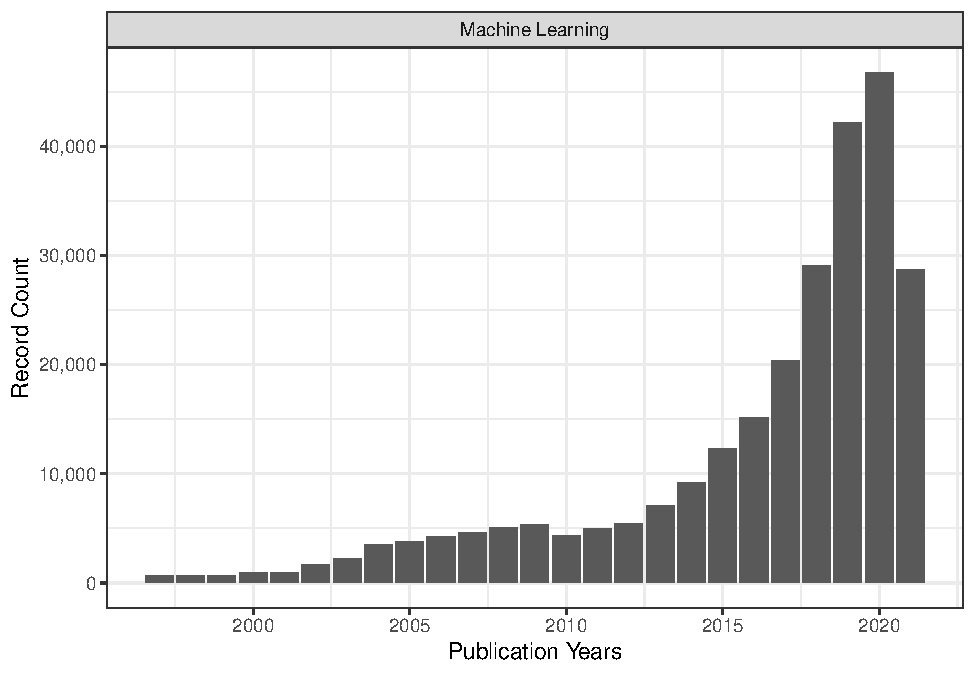
\includegraphics[width=0.49\linewidth]{main_files/figure-latex/wos-1} 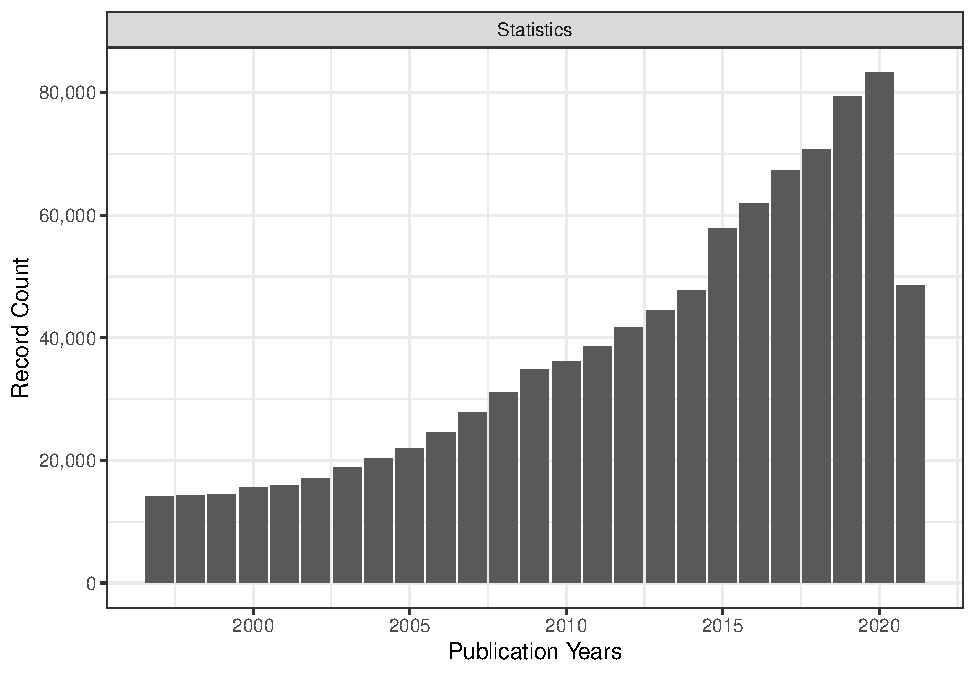
\includegraphics[width=0.49\linewidth]{main_files/figure-latex/wos-2} 

}

\caption{\textit{Left panel: Number of publications selected from the Web of Science Core Collection with the search term 'machine learning', per year. Right panel: Number of publications selected from the Web of Science Core Collection with the search term 'statistics', per year. Searches were carried out on 08/14/2021. Note that the year 2021 is incomplete.}}\label{fig:wos}
\end{figure}

We have showed that AI and ML are increasingly popular within research. AI and ML are also increasingly effective. This is not only because of the continuing development of new and better algorithms, but also because of advances in computing power and the ever increasing amounts of data that can be fed into these machine learning models. Indeed, a recent study showed empirically that model selection gets less important as training sets take on extreme proportions, suggesting that \emph{``{[}\ldots{]} the scientific community should perhaps focus more on data curation than on algorithm development''} (Halevy, Norvig, and Pereira 2009), {[}very\_large\_corpora{]}, (Géron 2020).

We are now in the era of `big data,' where the amount of data that are created is unimaginably high. However, while it is true that for example high-throughput technologies such as \textbf{single cell sequencing} produce huge amounts of data, knowledge extraction from these data sources still remains a difficult task. Why that is has to do with what is called the curse of dimensionality which is discussed in the following subsection.

\hypertarget{the-curse-of-dimensionality}{%
\subsection{The curse of dimensionality}\label{the-curse-of-dimensionality}}

In this thesis we want to focus on the analysis of data that are used for biomarker discovery within pre-clinical pharmaceutical research. In this field, the researcher is typically interested in finding results that ultimately will allow for quick and cost-effective identification or prediction of clinically relevant outcomes. Examples of such outcomes are the presence of a disease, the acceptance or rejection of a transplanted organ, the presence of severe side effects, etcetera. In this thesis we will focus on binary classification problems.

Biomarker candidates are typically found in `omics' data. This could be genomic, transcriptomic, proteomic etc. data or even a combination. The datasets in these settings are typically (ultra) high dimensional, i.e.~data where the number of features far exceeds the number of instances. This is often denoted as p \textgreater\textgreater{} n where p is the number of features and n is the number of samples. In the case of biomarker discovery research the dimensionality of datasets are typically in the range of thousands to ten thousands.

This high dimensionality introduces serious challenges for the analyst who wants to extract knowledge from these datasets. These challenges are often referred to as the \emph{curse of dimensionality}. The curse of dimensionality is called this way because there are a number problems that arise when the dimensionality of a dataset increases. More so, these problems get worse very quickly with further increasing dimensionality.

For many people, this could be counterintuitive as it apparently goes against what people remember from their statistics classes, that is: the adage that more data is better. The confusion could come from the faulty belief that `more dimensions' means the same as `more information.' While it is true that there are more entries in a 100-dimensional dataset than in a 10-dimensional dataset, for a constant number of instances there are, however, an equal amount of data points in both datasets. The reason this causes problems has to do with the geometry of high dimensional spaces. Two important reasons are briefly discussed below. This discussion is not meant to be exhaustive.

Firstly, as the dimensionality increases, the volume of the data-space increases exponentially. This means, with the same number of samples, an increase in dimensions leads to a sparser populated data-space compared to lower dimensions. The sampling density is proportional to \(n^{1/p}\), so one needs \(n^p\) samples in p-dimensional space in order to have the same sampling density as in one-dimensional space (Hastie, Tibshirani, and Friedman 2009). This is a problem because in realistic settings where the cost of biological samples is very high, one cannot gather much more data than 10 to 50, maybe at most 100 samples. Contrasting this number with the number of features (often thousands or more) shows that the data-space is immensely sparse populated. Lower sampling density will then result in higher variance of estimates and thus in decreased performance.

A second property of high dimensional space that is related to decreased performance of statistical methods is the fact that in high dimensional space most of the data-points are rather `extreme' in one way or another. Hastie, Tibshirani, and Friedman (2009) showed that the median distance from the origin to each of 500 uniformly distributed data-points in 10-dimensional unit space is more than halfway. They conclude that more than half of the points are closer to the boundary than to any other data point. This is a problem because prediction is much more difficult near the edges of the training space because that relies more on extrapolation rather than interpolation.

Now it is clear there are challenges with high dimensional data, we now shift our attention to different methods to analyze these kinds of data.

\hypertarget{methods-for-biomarker-discovery-with-high-dimensional-data}{%
\subsection{Methods for biomarker discovery with high dimensional data}\label{methods-for-biomarker-discovery-with-high-dimensional-data}}

In this thesis we want to compare 5 different statistical methods for the analysis of omics data in biomarker discovery. The selection of these methods was partially based on what is actually used in research departments of pharmaceutical companies (FDR, LASSO), partially on theoretical properties (Tweedie), and partially on a brief scan of the literature (Boruta, SVMRFE).

\hypertarget{intro-FDR}{%
\subsubsection{T-tests with false discovery rate control}\label{intro-FDR}}

The Welch t-test is a relatively simple method that is used to find out if 2 groups have different means at the population level. In the case of biomarker discovery one t-test for every feature is performed. Because of the vast amount of features in these kinds of datasets, this strategy without any adjustment is problematic. Typically a researcher wants to control the type-I error rate at a certain level (say 0.05). While Welch's t-test controls the type-I error well at the level of the individual test, the type-I error rate inflates when multiple tests are performed within one study at the level of the study which is more of interest. This well known phenomenon is known as the multiple testing problem. Apart from the inflation at the `family' level, there is also the practical problem of having on average 500 false positive results out of 10,000 comparisons (when the null hypothesis holds for every comparison).

A lot of strategies to cope with this problem have been proposed, of which Bonferroni correction is a well known example. Due to its very conservativeness that method is less suited for large scale hypothesis testing. Most often one choses not to control the family wise error rate but the false discovery rate (FDR) instead, and use the method of Benjamini and Hochberg (1995). There are other FDR methods but we will focus on Benjamini and Hochberg (1995).

This method is based on the knowledge that p-values that come from null-comparisons are uniformly distributed and that the distribution of p-values that come from true differences are skewed with a mode close to 0. This knowledge makes it possible to adjust the p-values so that only 5\% of the discoveries are expected to be false.

An example of a study that use this method is Marcišauskas et al. (2019).

\hypertarget{intro-Tweedie}{%
\subsubsection{T-tests with emperical Bayes based correction using Tweedie's formula}\label{intro-Tweedie}}

Selection bias is the phenomenon of overestimating population parameters based on extreme observations. This phenomenon is also known as regression to the mean. If one would throw many dice, we would expect the mean number of pips to be around 3.5. If one would then rethrow those dice that resulted a 6, the mean would again expected to be 3.5. This is an example of regression to the mean. The mean of the selected dice (6) regresses back to the overall mean (3.5). Expecting a higher mean would be an example of selection bias.

Efron (2011) describes Tweedie's formula as a means to deal with this selection bias. Tweedie's formula was introduced in Robbins (1956). It assumes that observations z have a true mean \(\mu\), come from a distribution \(N(\mu,\sigma^2)\) and that every \(\mu\) has an unknown prior distribution \(g(\mu)\). The formula is \(E\{\mu|z\} = z + \sigma^2l'(z)\) and an estimate \(\hat{\mu}\) can be obtained by applying following estimator: \(z + \sigma^2\hat{l'}(z)\)

where \(l'(z)\) is the first derivative of the marginal log-density of z, evaluated at z. Efron (2011) points out that the formula is practical because of the fact that one only needs an estimate of the marginal (log-) density of z, and no estimate of the prior. Efron (2011) suggests estimating the log-density by applying Lindsey's method. Lindsey's method is described in Efron (2008) and comes down to fitting a Jth degree polynomial poisson regression to the counts of the observations z in a number of bins. In other words, Lindsey's method tries to fit a Jth degree polynomial to a histogram. Because the Jth degree polynomial is of form \(f(z) = exp\{\sum^J_{j=0}\beta_jz^j\}\), it is convenient to take the logarithm and calculate the derivative from there (Efron 2011).

Efron (2011) shows there is a connection between Tweedie's formula and the FDR method of Benjamini and Hochberg (1995) and the local false discovery rate.

Because of the selection-bias eliminating characteristics of Tweedie's formula it is interesting to see how it performs next to more popular methods such as FDR control and LASSO.

To our knowledge no implementation of the above is available in the form of R-code so one aim of this thesis is to implement this ourselves.

\hypertarget{intro-LASSO}{%
\subsubsection{L1-penalized logistic regression}\label{intro-LASSO}}

Logistic regression is a commonly used method to model the conditional probability of an observation belonging to one group (vs.~an other group), given the values of the independent variables for that observation. That model and its probability as output is then often used to make predictions on the group status of new observations.

The benefits of regularization are well known and include among others protection against overfitting which is especially of importance in high dimensional settings. Different kinds of regularization are known among which L1-penalization or LASSO is a popular choice. LASSO, introduced in Tibshirani (1996), adds an L1-norm penalty term to the loss function (which is log loss for logistic regression) which penalizes large values for the coefficients and effectively shrinks them towards 0. Note that the intercept is kept out of this term and thus does not contribute to the penalization. A penalization parameter \(\lambda\) is introduced to allow control of the amount of penalization. This parameter can vary from 0 (which results in no regularization) to infinity (which results in a model with only an intercept) and can be chosen through cross validation.

The extra benefit of the LASSO compared to for example L2-norm penalization is that it not only shrinks coefficients towards 0, it also sets some coefficients at exactly 0. As a result, LASSO usually results in a more parsimonious model as it `selects' only those features that are deemed necessary. For this reason, this method is attractive for use in biomarker discovery.

\hypertarget{intro-Boruta}{%
\subsubsection{Boruta}\label{intro-Boruta}}

Boruta (Kursa and Rudnicki 2010) is a random forest based feature selection method. Random forest (L 2001) is a method in which an ensemble of decision trees, in which each tree is built on a bootstrap sample of the original dataset and in which at each branch only a random subset of the variables are considered. In each ensemble, a fixed number of random trees are built, hence `random forest.' A property of the random forest algorithm is that it introduces repeated randomness to mitigate the fact that a single decision tree is a high variance method.

The Boruta method works as follows. For each feature in the dataset a `shadow' feature is created. These shadow features are copies of the original features that are shuffled across samples. Once the shadow features are added to the dataset, a random forest is fitted. The variable importance of every feature is then evaluated against the mean shadow feature importance. This process is then repeated until all features are either categorized important or unimportant or until a certain number of runs is reached.

\hypertarget{intro-SVMRFE}{%
\subsubsection{Support vector machine recursive feature elimination}\label{intro-SVMRFE}}

Support vector machine recursive feature elimination (SVMRFE) is method that consists of iteratively fitting a support vector machine model to correctly classify the subjects. At the end of each iteration the variables with the lowest variable importance are discarded from the feature pool before a new iteration begins.

Support vector machines are a family of models that, for classification, try to find a maximally separating hyperplane between two classes in the data space. An other way to look at support vector machines is that they minimize hinge loss. To avoid severe overfitting, a form of regularization is used (L2 penalization). In using support vector machines, one needs to choose a kernel. In the simulation study we used a linear kernel.

\newpage

\hypertarget{methods}{%
\section{Methods}\label{methods}}

In this section we follow the guidelines of Morris et al.~in that we structure the methods section according to the ADEMP acronym, which stands for aims, data-generating mechanisms, estimands or targets, methods, and performance measures.

\hypertarget{aims}{%
\subsection{Aims}\label{aims}}

We want to examine, by means of a simulation study, several properties of the 5 aforementioned methods in the context of pre-clinical pharmacological research where high dimensional (omics) data on only very few subjects are to be analyzed. These properties are:

\begin{itemize}
\item
  the mean number of true / false detections
\item
  the chance of doing at least one true / false detection
\item
  the rate of null-results
\item
  the duration of the analysis
\item
  discriminative ability for the model based methods
\end{itemize}

In doing so we hope to identify:

\begin{itemize}
\item
  conditions under which the methods under investigations fail or break or, as we call it, boundary conditions
\item
  relative strengths
\end{itemize}

\hypertarget{data-generating-mechanisms}{%
\subsection{Data-generating mechanisms}\label{data-generating-mechanisms}}

We will simulate data using a simple parametric model (normal distribution) that will allow to manipulate the data easily.

We will consider a number of different scenario's for this simulation study. To this end we will vary:

\begin{itemize}
\item
  the number of subjects, n
\item
  the number of features, p
\item
  the number of significant features, sig\_p
\item
  the difference in population mean between the 2 groups for the significant features, or effect size, d
\item
  correlation structure
\end{itemize}

We have simulated a number of different scenarios using a low number of repetitions to explore which parameter settings yield the most interesting results. These can be found in appendix \ref{exploratory}. From this first round of simulations we could select scenarios in a more informed manner. These scenarios were then simulated one hundred times.

In each scenario there will be 2 groups (k, treatment vs.~control) of equal size. In the scenarios with no correlation between features, the data will be simulated following \$ X\_\{ij\}\^{}\{k\}\$ distributed as \(N(k \delta_j, 1)\), with i = 1 \ldots{} n, j = 1 \ldots{} p, k = 0, 1 and \(\delta_j = d\) for j = 1\ldots sig\_p and \(\delta_j = 0\) for j = sig\_p+1\ldots p.~

In the scenarios with correlation we use a block correlation structure for the correlation matrix following the same architecture as in Acharjee et al. (2020), that is 6 groups of 10 features that are highly intra-group correlated and a seventh rest group with no correlation (see figure \ref{fig:blockcor}). To achieve the block correlation structure we use the simcor function from the MarkJBrewer/ICsims package (Brewer, n.d.). The intra-group correlations were set at 0.9, the other correlations were set at 0.

\begin{figure}

{\centering 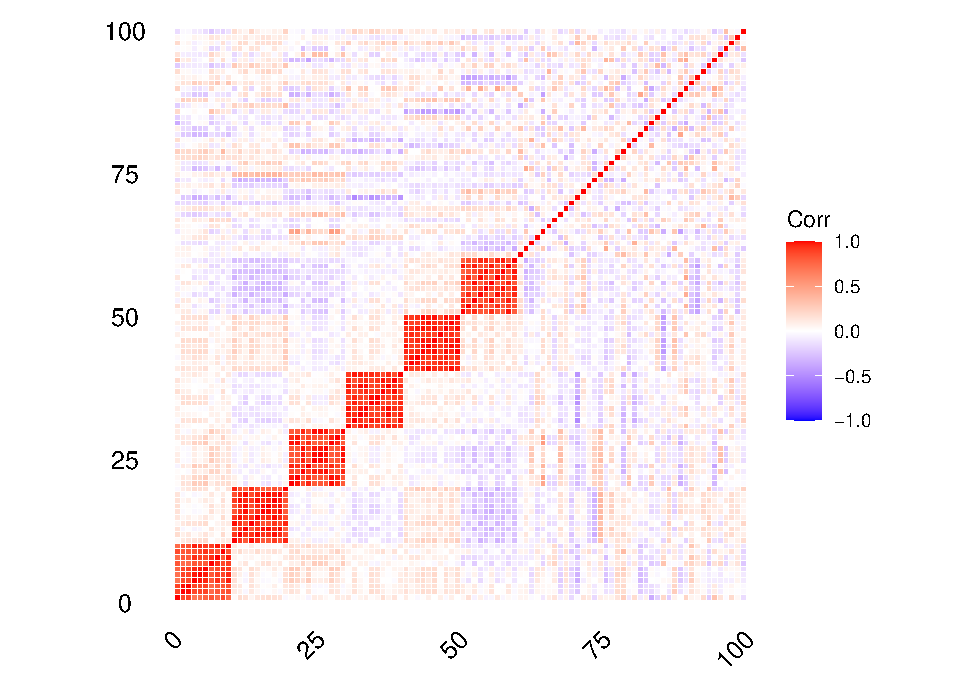
\includegraphics[width=0.75\linewidth]{main_files/figure-latex/blockcor-1} 

}

\caption{\textit{First 100 features of an example of the block correlation structure used in the correlated scenarios.}}\label{fig:blockcor}
\end{figure}

\hypertarget{targets-and-performance-measures}{%
\subsection{Targets and performance measures}\label{targets-and-performance-measures}}

The statistical task we are evaluating the methods on is model selection (for the models) and hypothesis testing (for the t-tests). We want to measure how good the methods can discriminate between significant and non-significant features. We want as many true positives as possible while keeping the false positives as low as possible.

The performance measures we are using are the mean number of true/false detections and the chance of true/false detection. Additionally we are also measuring the rate of null-results, and the duration of the analyses. We define null-results as results with no positives, true or false.

The discriminative ability of the model based methods will be measured with the AUC. After the feature selection, a model will be built with those features. That model will then be tested on a separate test set (see below). LASSO will just use its output model. Boruta results in a random forest model, and SVM-RFE results in a SVM.

\hypertarget{implementation-of-methods}{%
\subsection{Implementation of methods}\label{implementation-of-methods}}

This sections discusses the practicalities of the implementation of the different methods, allowing reproducibility. For a substantive discussion of the methods, please refer to sections \ref{intro-FDR} to \ref{intro-SVMRFE}.

We have 3 model based methods and 2 hypothesis test based methods. The hypothesis test based methods are performed using all available data. In the case of the model based methods, a separate train and test set is created using a 1:2 ratio (2/3 train set, 1/3 test set). This train-test split is done to reflect real life analyses and the 1/3 test set size is chosen because the more standard 20\% test split size did not work in the scenarios with sample size of 10.

\hypertarget{t-tests-with-false-discovery-rate-control}{%
\subsubsection{T-tests with false discovery rate control}\label{t-tests-with-false-discovery-rate-control}}

In a first step the p t-tests are performed. Then, the corrections to the p-values are made, turning them into q-values, using the p.adjust function and using the BH (Benjamini and Hochberg 1995) method. After this correction, each feature for which holds that the q-value \textless{} 0.05 is stored as a detection.

\hypertarget{t-tests-with-tweedie-correction}{%
\subsubsection{T-tests with Tweedie correction}\label{t-tests-with-tweedie-correction}}

In a first step the p t-tests are performed. Each test statistic is stored and is binned into one of 30 bins. The number of test statistics per bin is counted. This comes essentially down to creating a histogram of the test statistics. Then a 5th degree polynomial poisson regression is fitted with the counts as dependent an the middle of each bin as independent variable. The result is a model that approximates the empirical probability density function of the test statistics. In a next step the variance of the test statistics is estimated and the derivative of the approximated density function is evaluated for each test statistic. At this point we have everything needed to apply Tweedie's formula \(E\{\mu|z\} = z + \sigma^2l'(z)\) and we calculate the corrected test statistics and according p-values. Each feature for which holds that the p-value \textless{} 0.05 is stored as a detection.

\hypertarget{l1-penalized-logistic-regression}{%
\subsubsection{L1 penalized logistic regression}\label{l1-penalized-logistic-regression}}

L1 penalized logistic regression has a hyperparameter (the penalization parameter \(\lambda\)) that needs to be tuned. The preffered way to do this is to do a grid search of possible values for \(\lambda\) in conjunction with cross validation. We did a 5-fold cross validation with the cv.glmnet function of the glmnet package (Tibshirani 1996), using the AUC as criterion. The cv.glmnet function provides parallel support which was used for p \textgreater{} 1000. This threshold was chosen after initial experimentation and profiling of the code. Once the optimal value for \(\lambda\) was chosen, i.e.~the minimal value for lambda for which the AUC is maximized, a final model was fitted with this value for \(\lambda\). The selected features were then stored as detections.

A construction to catch errors was necessary for the scenarios with extreme small sample sizes (10) because in those cases it happens that some folds have 0 observations in one of the 2 classes.

\hypertarget{boruta}{%
\subsubsection{Boruta}\label{boruta}}

Boruta is very easy to implement. The Boruta package (Kursa and Rudnicki 2010) provides a Boruta function to which you can pass the data and several other parameters. We set the critical p-value at 0.05 and the number of trees at 500. Only features that had a ``confirmed'' status after the algorithm was finished were treated as detected features.

\hypertarget{svmrfe}{%
\subsubsection{SVMRFE}\label{svmrfe}}

We used a variant of SVMRFE which uses cross validation to achieve more stability. As with the L1 penalized logistic regression we chose to do a 5-fold cross validation. To speed up the computation, it is possible to tell the algorithm to halve the number of features each iteration until a certain number of features is reached. We chose a number (250) that was not too high, so that we could effectively speed up the computation, nor too low, so that the risk of accidentally eliminating significant features early on was kept at a minimum. As the algorithm gives a ranking of the features it was necessary to employ a rule to select the features. Based on Heinemann et al. (2014) we chose to select the top 1\% as detections.

\hypertarget{software-reproducibility-and-code-availability}{%
\subsection{Software, reproducibility, and code availability}\label{software-reproducibility-and-code-availability}}

The simulations and analyses were programmed in R v4.1.1 (R Core Team 2021). The packages that were used for the different methods are listed in table \ref{tab:packages}. To ensure reproducibility a different seed was used for the pseudo random number generator. These seeds are listed in in table \ref{tab:seeds}. For reproducibility purposes, the session info can be found in appendix \ref{sessioninfo}.

\begin{table}

\caption{\label{tab:packages}Used packages related to methods}
\centering
\begin{tabular}[t]{lll}
\toprule
Method & Package & Citation\\
\midrule
Boruta & Boruta & Kursa and Rudnicki (2010)\\
Logistic LASSO & glmnet & Friedman, Hastie, and Tibshirani (2010)\\
SVMRFE & SVM-RFE & Duan et al. (2005)\\
\bottomrule
\end{tabular}
\end{table}

T-tests and FDR adjustment (Benjamini and Hochberg 1995) are implementen in base R. The Tweedie-correction has, to our knowledge, no implementation and has been programmed by the author.

\begin{table}

\caption{\label{tab:seeds}Used seed per scenario}
\centering
\begin{tabular}[t]{llllll}
\toprule
scenario & correlated & d & sig\_p & n & seed\\
\midrule
A1 & no & 1.1 & 10 & 50 & 2108191137\\
A2 & no & 0.7 & 10 & 50 & 2108191339\\
A3 & no & 0.3 & 10 & 50 & 2108191522\\
B1 & no & 0.9 & 1 & 10 & 2108191717\\
B2 & no & 1.81 & 1 & 10 & 2108191839\\
\addlinespace
C1 & no & 0.95 & 3 & 30 & 2108191954\\
C2 & no & 1.3 & 3 & 30 & 2108200747\\
D & no & 0 & 0 & 20 & 2108201715\\
block A1 & block & 1.1 & 10 & 50 & 2108201412\\
block C2 & block & 1.3 & 3 & 30 & 2108201023\\
\bottomrule
\end{tabular}
\end{table}

\newpage

\hypertarget{results}{%
\section{Results}\label{results}}

Ten scenarios are presented in this results section. An overview of the different scenarios can be seen in figure \ref{fig:overviewscenarios}.

\begin{figure}

{\centering 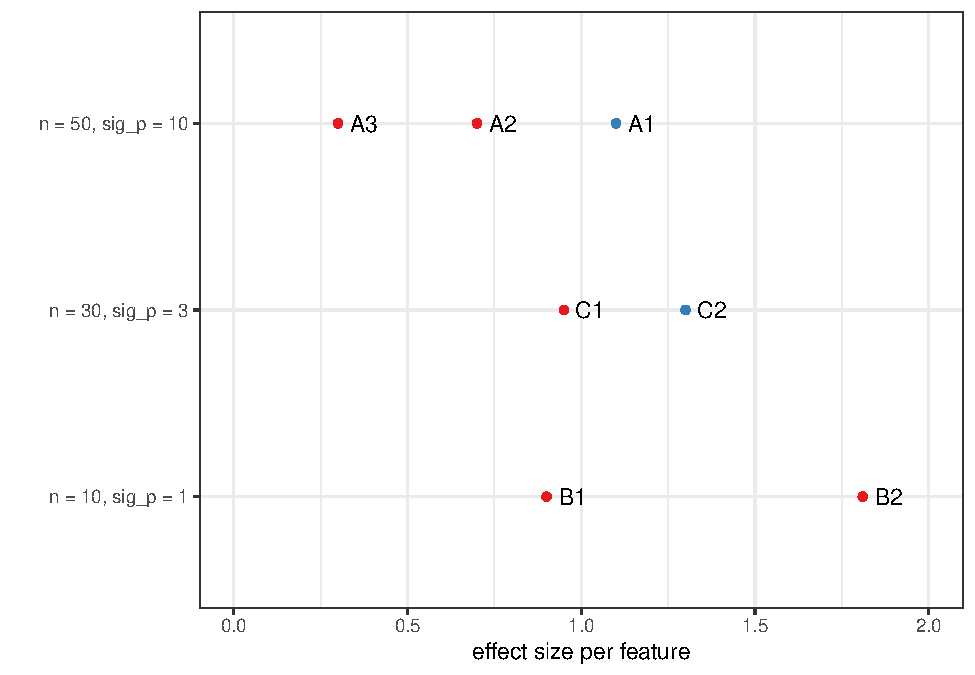
\includegraphics[width=0.75\linewidth]{main_files/figure-latex/overviewscenarios-1} 

}

\caption{\textit{Overview of the different scenarios. Blue dots: Scenarios was performed with and without correlation structure. Red dots: Scenario was only performed without correlation structure.}}\label{fig:overviewscenarios}
\end{figure}

\hypertarget{scenarios-a---optimistic}{%
\subsection{Scenarios A - Optimistic}\label{scenarios-a---optimistic}}

All scenarios `A' are `optimistic' scenarios in that they are scenarios with relatively many samples (50) and relatively many significant features (10) and no correlations between features. Within this optimistic setting, 3 different effect sizes are considered.

\hypertarget{scenario-a1}{%
\subsubsection{Scenario A1}\label{scenario-a1}}

The first effect size considered is relatively large (d = 1.1, or AUC = 0.78), yet not overly large so that all methods would perform equally well. The results can be seen in figure \ref{fig:A1}.

In terms of mean number of false discoveries SVM performs the worst and shows a different behavior than most other methods with respect to growing number of features p.~SVM shows a linear increase of mean number of false discoveries with growing number of features, on a logarithmic scale, whereas LASSO, Tweedie, and FDR stay relatively stable across number of features, or even show a decrease (FDR). Boruta, like SVM, shows a linear increase in mean number of false discoveries with growing p, though less pronounced. The best performing method is FDR with mean number of false discoveries less than 1 throughout the entire range of p.~

In terms of chance of discoveries we can more or less draw the same conclusions. That is, with regard to false discoveries FDR is the best performing method. SVM and Boruta are the worst performing methods.

With respect to null results we see that FDR and LASSO are more prone to delivering null results than the other methods.

For the model based method we calculated the AUC of the models trained on the training set and tested on the test set. We can see that LASSO is consistently better than the other 2 methods.

\begin{center}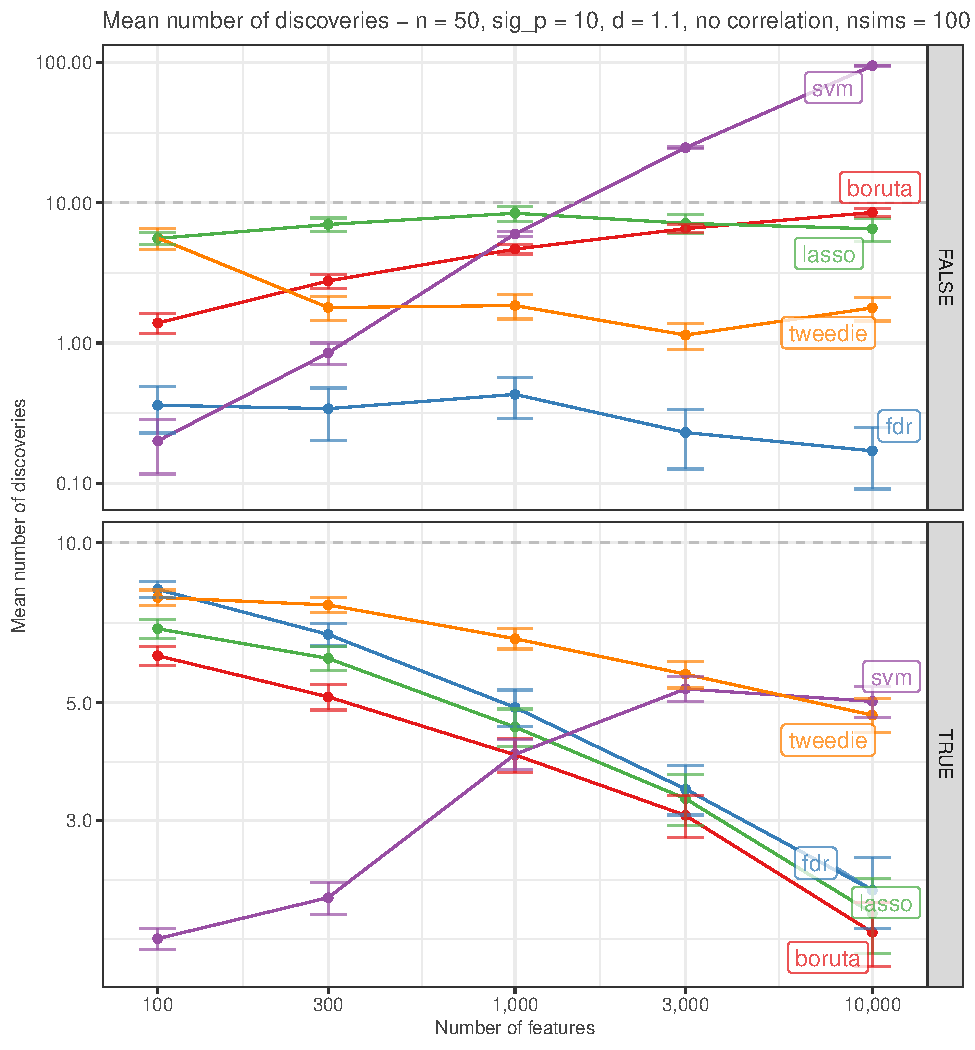
\includegraphics[width=0.49\linewidth]{main_files/figure-latex/unnamed-chunk-40-1} 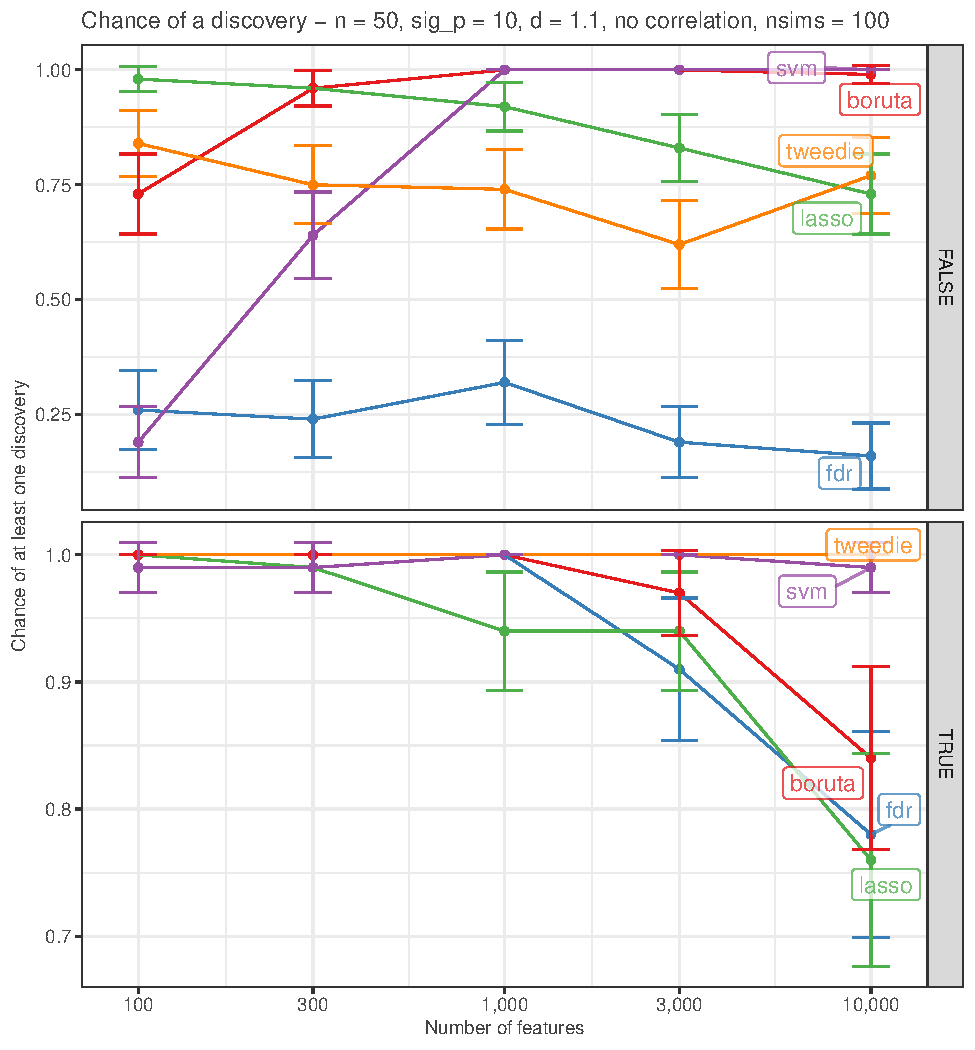
\includegraphics[width=0.49\linewidth]{main_files/figure-latex/unnamed-chunk-40-2} \end{center}

\begin{figure}

{\centering 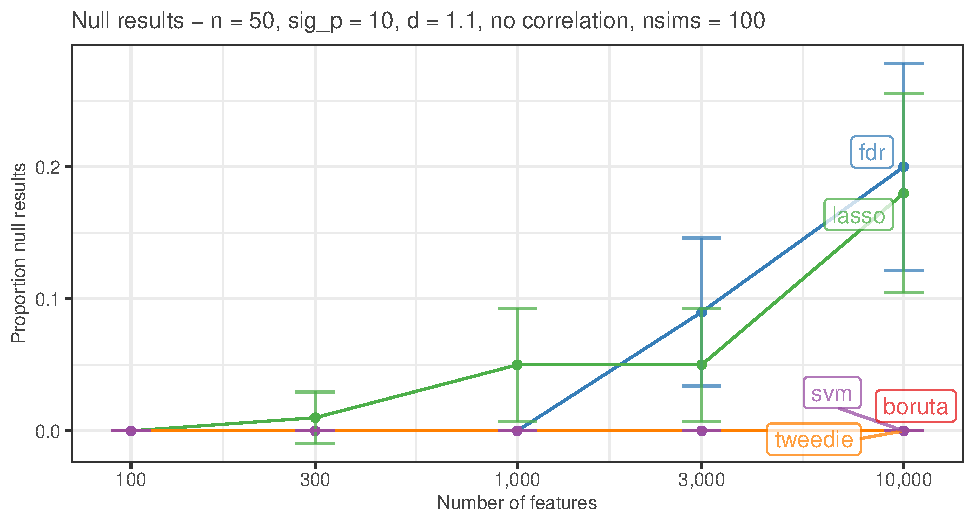
\includegraphics[width=0.49\linewidth]{main_files/figure-latex/A1-1} 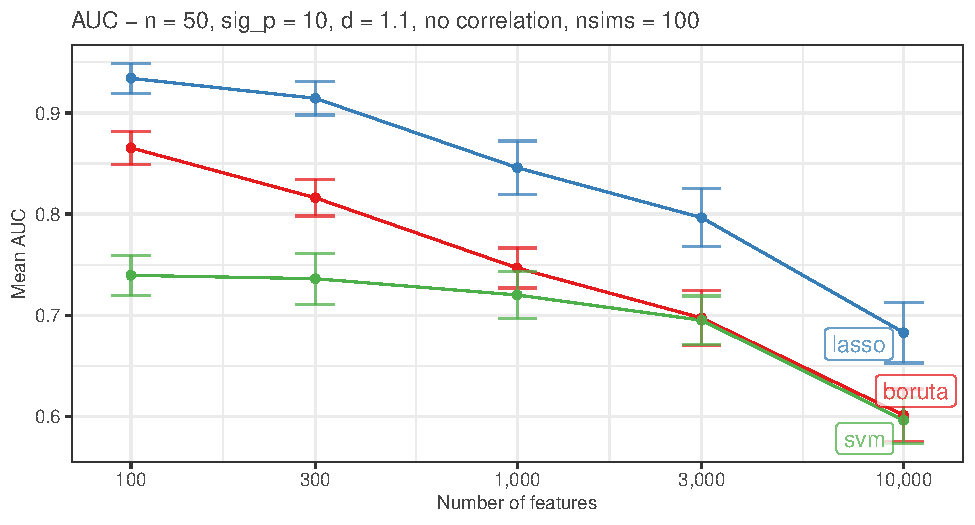
\includegraphics[width=0.49\linewidth]{main_files/figure-latex/A1-2} 

}

\caption{\textit{Upper left: Mean number of false and true discoveries for various numbers of features for every method. Upper right: Chance of at least one false and true discovery for various numbers of features for every method. Bottom left: Proportion of null results for various numbers of features for every method. Bottom right: Mean AUC of models built on selections by the model based methods for various numbers of features. 95\% confidence intervals are shown. In the case an interval is lacking, this has to do with the log scale of some of the plots.}}\label{fig:A1}
\end{figure}

\hypertarget{scenario-a2}{%
\subsubsection{Scenario A2}\label{scenario-a2}}

In this scenario the effect size is 0.7 (or AUC = 0.69) per feature. This scenario reflects slightly worse than optimistic conditions. The results can be seen in figure \ref{fig:A2}.

In terms of mean number of false discoveries SVM again performs the worst, while FDR is again the best method. In between lies (in order from better to worse) Tweedie, LASSO and Boruta. In terms of mean number of true discoveries we see again SVM as the best method and FDR as the worst. It is worth noting that SVM is the only method with more than 1 mean true discovery in the p = 10,000 condition. This translates to the same pattern of chances of at least one discovery, which is close to 1 for SVM but under 0.5 for all other methods (for p = 10,000). Leaving SVM out of the discussion, Tweedie is consistently among the best methods throughout the entire range of p, with Boruta as a close contender.

In terms of chance of false discoveries we see that SVM and Boruta are the worst methods and FDR is the best method.

In terms of null results we can see that FDR is the worst method across all values for p.~LASSO does a better job but still has a considerable amount of null results. Tweedie has yet a smaller amount of null results, except at p = 10,000 where the amount of null results is the same as for LASSO. Boruta and SVM delivered the least number of null results.

In terms of discriminative ability the LASSO performs better than the other methods for low numbers of p (100, 300). For larger numbers of features the performances are very close with a slight advantage for SVM.

\begin{center}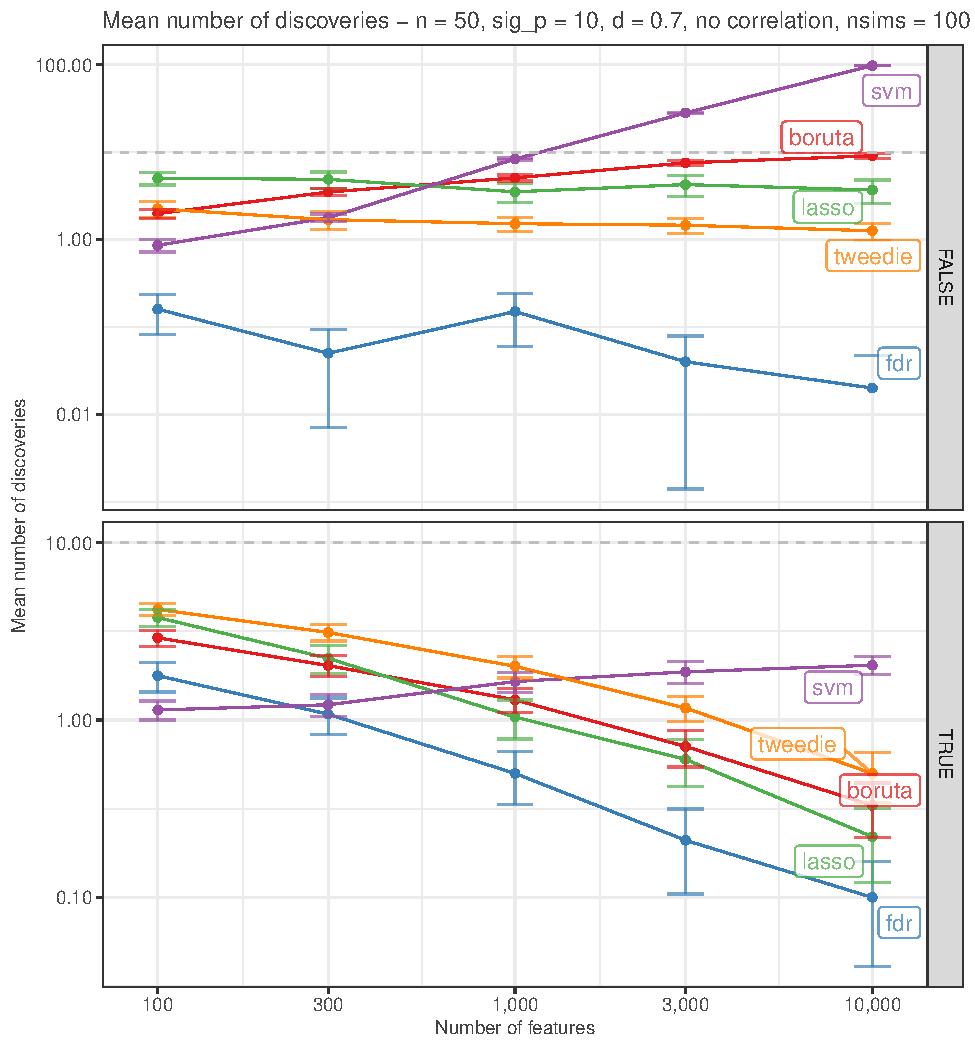
\includegraphics[width=0.49\linewidth]{main_files/figure-latex/unnamed-chunk-41-1} 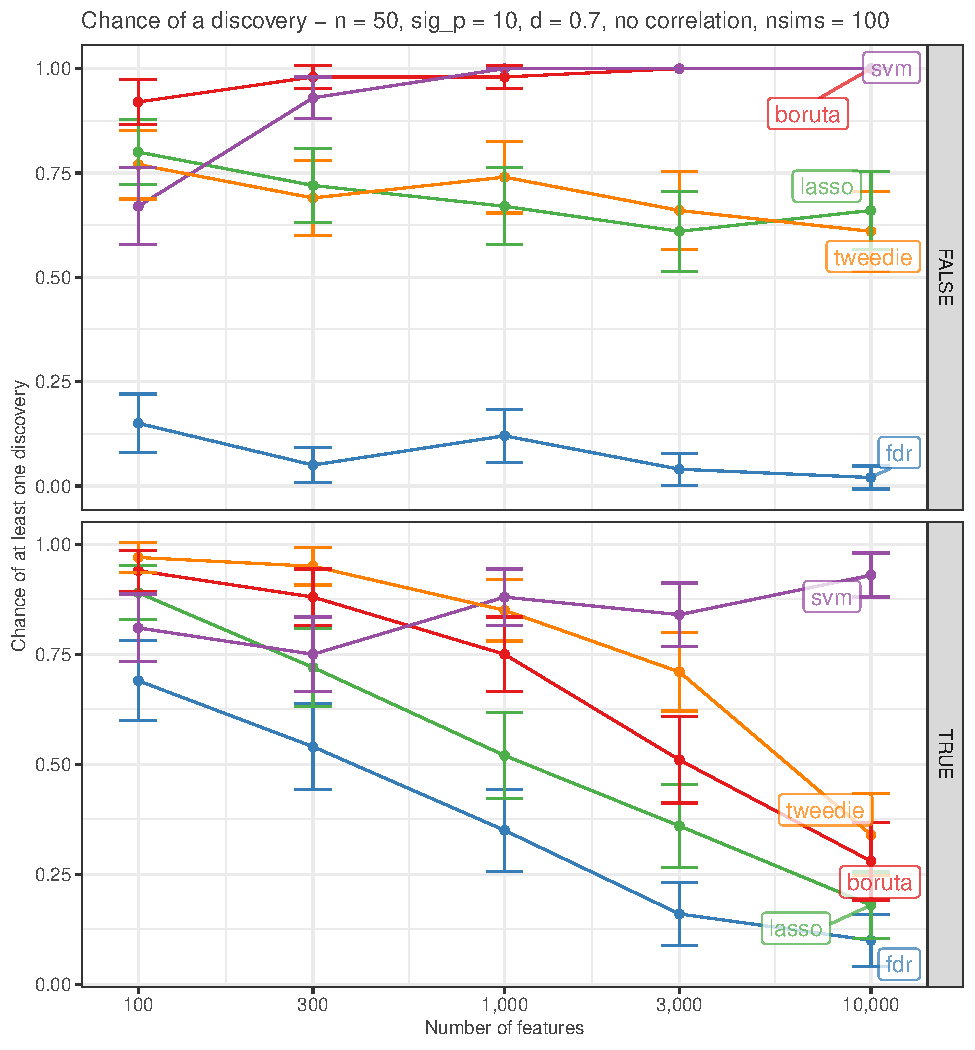
\includegraphics[width=0.49\linewidth]{main_files/figure-latex/unnamed-chunk-41-2} \end{center}

\begin{figure}

{\centering 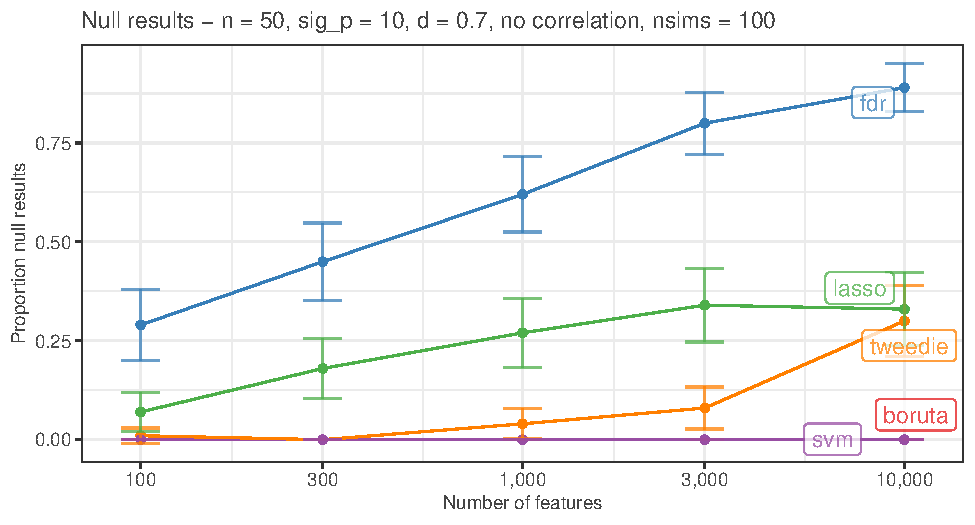
\includegraphics[width=0.49\linewidth]{main_files/figure-latex/A2-1} 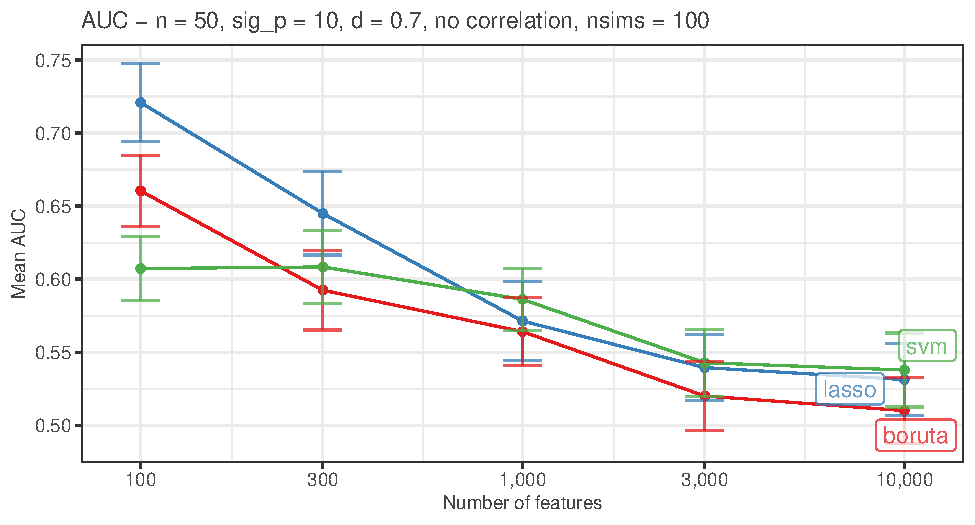
\includegraphics[width=0.49\linewidth]{main_files/figure-latex/A2-2} 

}

\caption{\textit{Upper left: Mean number of false and true discoveries for various numbers of features for every method. Upper right: Chance of at least one false and true discovery for various numbers of features for every method. Bottom left: Proportion of null results for various numbers of features for every method. Bottom right: Mean AUC of models built on selections by the model based methods for various numbers of features. 95\% confidence intervals are shown. In the case an interval is lacking, this has to do with the log scale of some of the plots.}}\label{fig:A2}
\end{figure}

\hypertarget{scenario-a3}{%
\subsubsection{Scenario A3}\label{scenario-a3}}

In this scenario the effect size is brought down to only 0.3 (or AUC = 0.58) per feature. This scenario reflects a boundary condition in which most methods fail to deliver any useful results. The results can be seen in figure \ref{fig:A3}.

In terms of mean number of false discoveries we again see that SVM performs worst and FDR performs best. SVM is again the best performing method and FDR the worst in terms of mean number of true discoveries. It is interesting to see that under these poor conditions (small effect size) SVM shows a stable performance across all values for p.~However, this performance is relatively poor (0.3, SE 0.05 at p = 10,000), indicating that this order of magnitude of effect size may represent a boundary.

More or less the same pattern of results can be seen in the results regarding chances of at least one detection. That is SVM and Boruta are the least performing methods with regard to false discoveries, and FDR is the best performing method. With regard to chance of at least one discovery SVM is the best performing method while all the other methods perform equally bad. Again the caveat about the relativity of what `best performing' means should be made. With a chance of at least one true discovery of 0.26 (SE 0.04) one could argue this is not a good performance at all.

With respect to null results FDR is again the worst method with consistently values larger than 0.75 across the values for p.~SVM and Boruta have the least null-results.

For the model based method we calculated the AUC of the models trained on the training set and tested on the test set. We can see that for almost all values for p, no model has an AUC higher than 0.5. Although only marginally relevant, the only exception is Boruta at p = 300 with.

\begin{center}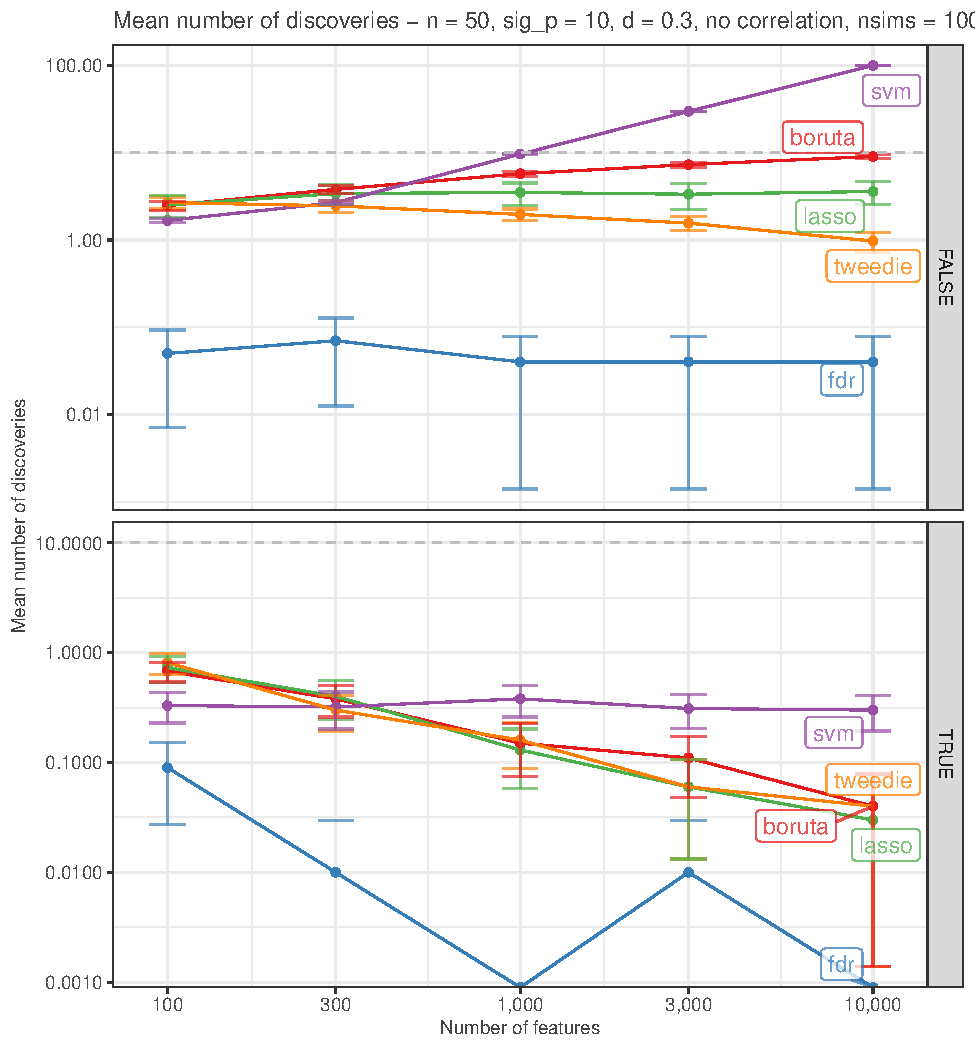
\includegraphics[width=0.49\linewidth]{main_files/figure-latex/unnamed-chunk-42-1} 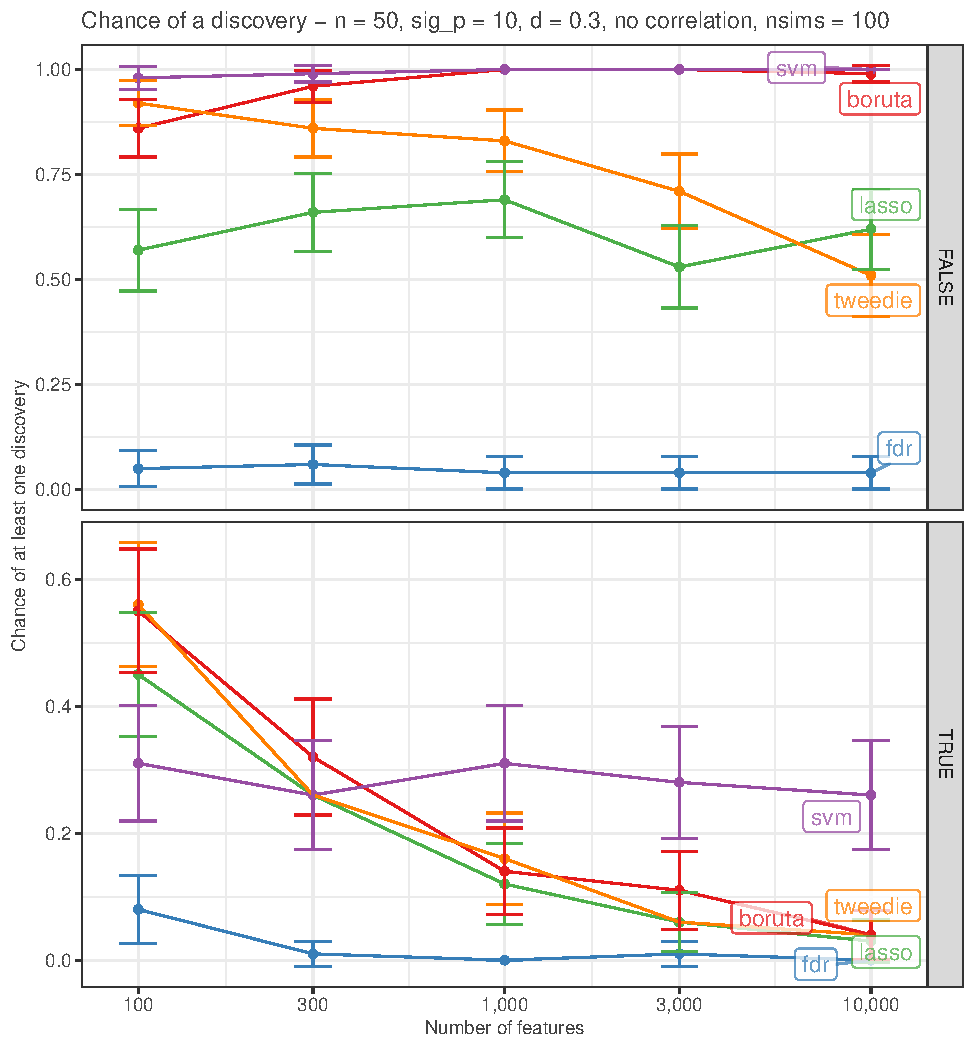
\includegraphics[width=0.49\linewidth]{main_files/figure-latex/unnamed-chunk-42-2} \end{center}

\begin{figure}

{\centering 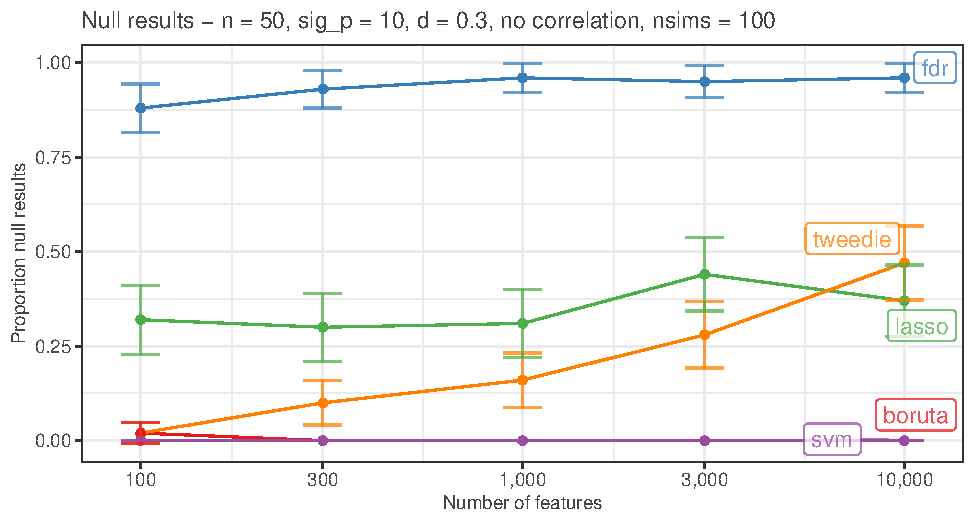
\includegraphics[width=0.49\linewidth]{main_files/figure-latex/A3-1} 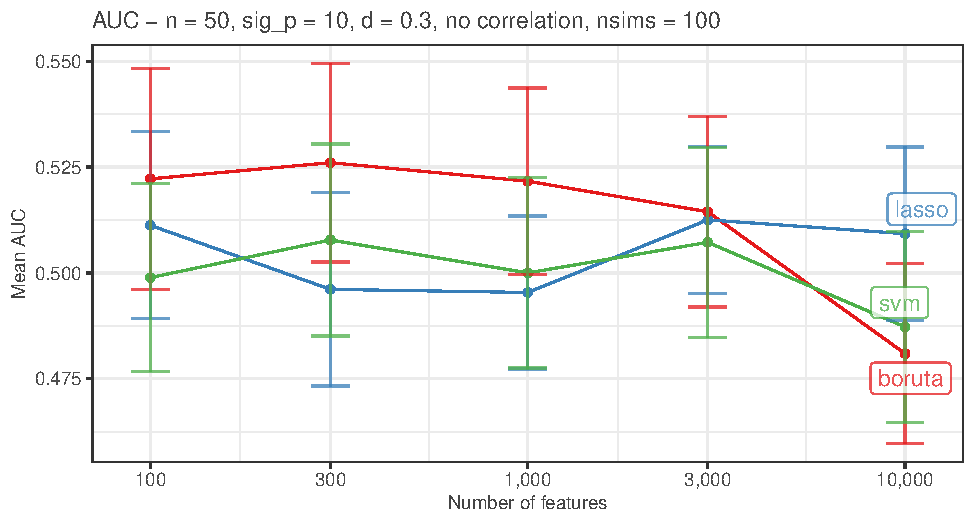
\includegraphics[width=0.49\linewidth]{main_files/figure-latex/A3-2} 

}

\caption{\textit{Upper left: Mean number of false and true discoveries for various numbers of features for every method. Upper right: Chance of at least one false and true discovery for various numbers of features for every method. Bottom left: Proportion of null results for various numbers of features for every method. Bottom right: Mean AUC of models built on selections by the model based methods for various numbers of features. 95\% confidence intervals are shown. In the case an interval is lacking, this has to do with the log scale of some of the plots.}}\label{fig:A3}
\end{figure}

\hypertarget{scenarios-b---pessimistic}{%
\subsection{Scenarios B - Pessimistic}\label{scenarios-b---pessimistic}}

All scenarios `B' are `pessimistic' scenarios in that they are scenarios with relatively few samples (10) and relatively few significant features (1) and no correlations between features. Within this pessimistic setting, 2 different effect sizes are considered.

\hypertarget{scenario-b1}{%
\subsubsection{Scenario B1}\label{scenario-b1}}

This scenario the effect size is relatively moderate (0.9, or AUC = 0.74) per feature. The results can be seen in figure \ref{fig:B1}.

One major observation is that Boruta totally fails in this scenario, that is it never yields any discoveries regardless of their status (true or false). In a way it is the least performing method overall. However, in the current section we will make a further distinction and discuss the best and worst methods among the other 4 methods.

With respect to mean number of false discoveries FDR is the best and SVM the least performing method. In terms of mean number of true discoveries Tweedie and SVM are the best performing methods. FDR and LASSO are virtually at the same level as Boruta (that is no true discoveries) for the entire range of p.~Although Tweedie and SVM are the best performing methods, they don't perform well with their mean below 0.1. This poor performance is reflected by the chance of true discovery that is below 0.1 for both methods, which means this scenario is indicative of a boundary condition.

In terms of null results FDR delivers poor results with a proportion of null results above of 0.9. Tweedie and SVM show the best results in this regard.

The model based methods perform poorly in terms of predictive ability with all AUC not different from 0.5.

\begin{center}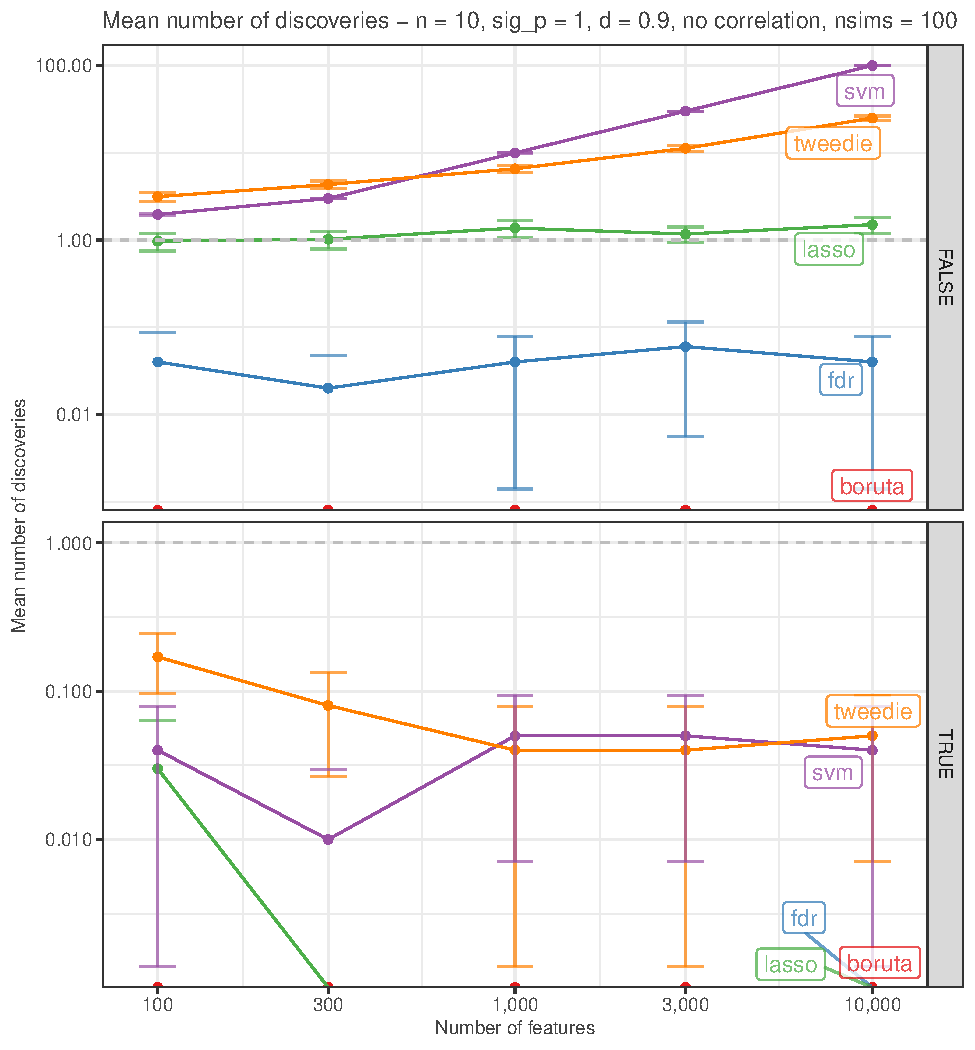
\includegraphics[width=0.49\linewidth]{main_files/figure-latex/unnamed-chunk-43-1} 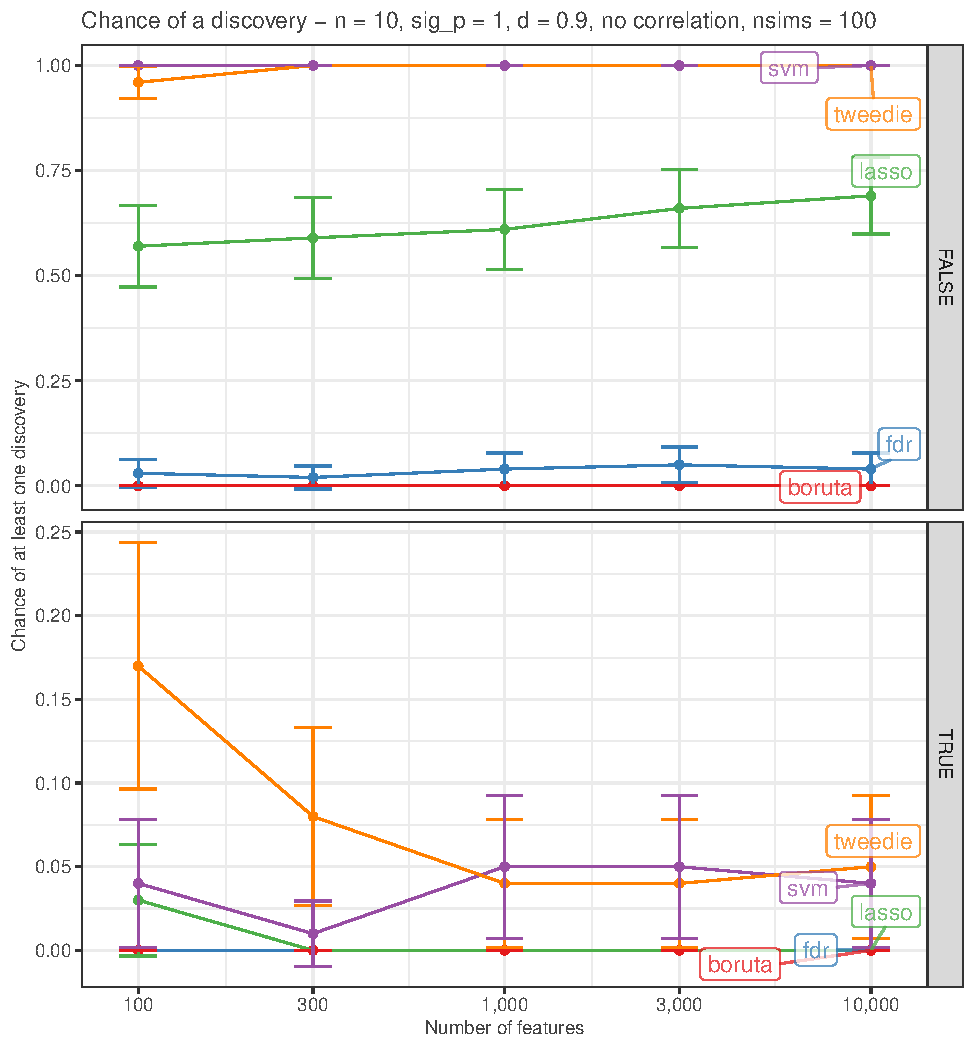
\includegraphics[width=0.49\linewidth]{main_files/figure-latex/unnamed-chunk-43-2} \end{center}

\begin{figure}

{\centering 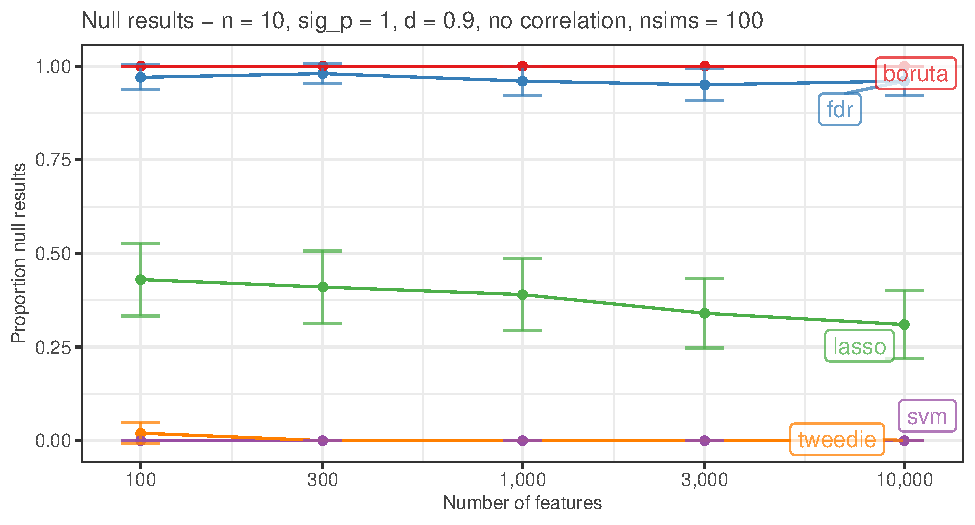
\includegraphics[width=0.49\linewidth]{main_files/figure-latex/B1-1} 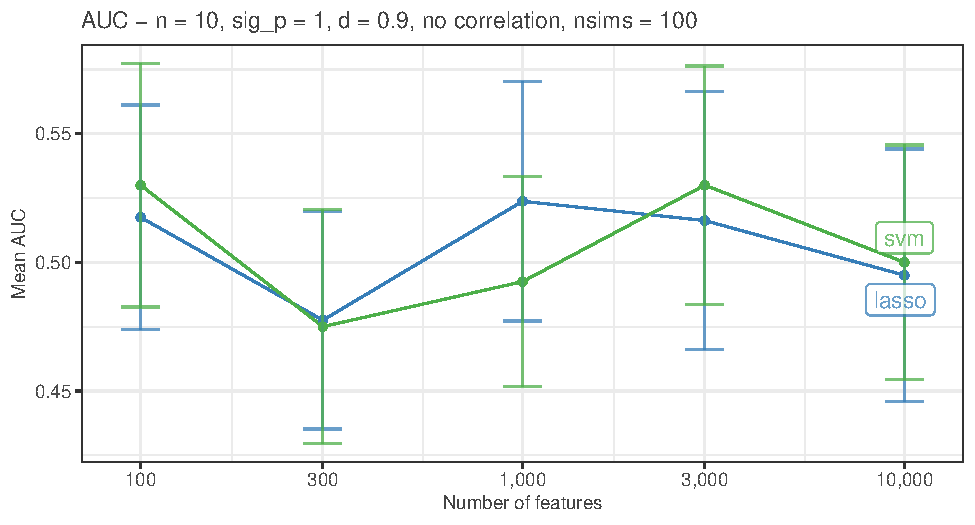
\includegraphics[width=0.49\linewidth]{main_files/figure-latex/B1-2} 

}

\caption{\textit{Upper left: Mean number of false and true discoveries for various numbers of features for every method. Upper right: Chance of at least one false and true discovery for various numbers of features for every method. Bottom left: Proportion of null results for various numbers of features for every method. Bottom right: Mean AUC of models built on selections by the model based methods for various numbers of features. 95\% confidence intervals are shown. In the case an interval is lacking, this has to do with the log scale of some of the plots.}}\label{fig:B1}
\end{figure}

\hypertarget{scenario-b2}{%
\subsubsection{Scenario B2}\label{scenario-b2}}

This scenario the effect size is relatively large (1.81, or AUC = 0.9) per feature. This scenario tries to mimic a best case of worst case scenarios. The results can be seen in figure \ref{fig:B2}.

Again we see that Boruta totally fails in this scenario. The same remark as in the previous scenario is made, that is that although Boruta is evidently the least performing method overall we will make a further distinction and discuss the best and worst methods among the other 4 methods.

In terms of mean number of false discoveries FDR is again the best performing method and SVM the worst performing method. In terms of true discoveries Tweedie and SVM are the best performing methods while FDR and LASSO perform the least. The mean number of true discoveries for the best methods is small (less than 0.2).

In terms of number of null results we see that, apart from Boruta, FDR is the method with the most null results while Tweedie and SVM are the methods with the least number of null results.

The model based methods were evaluated on their predictive ability. However, all mean AUC values are not different from 0.5.

\begin{center}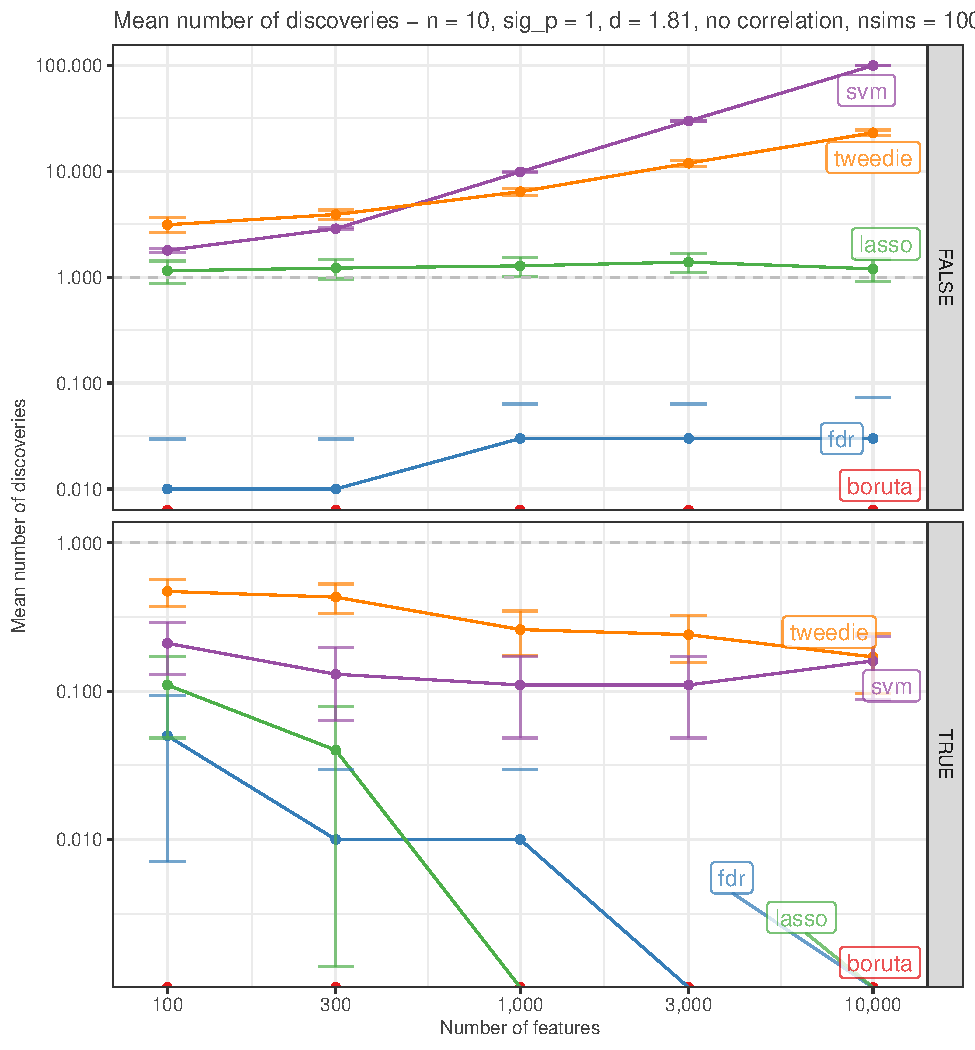
\includegraphics[width=0.49\linewidth]{main_files/figure-latex/unnamed-chunk-44-1} 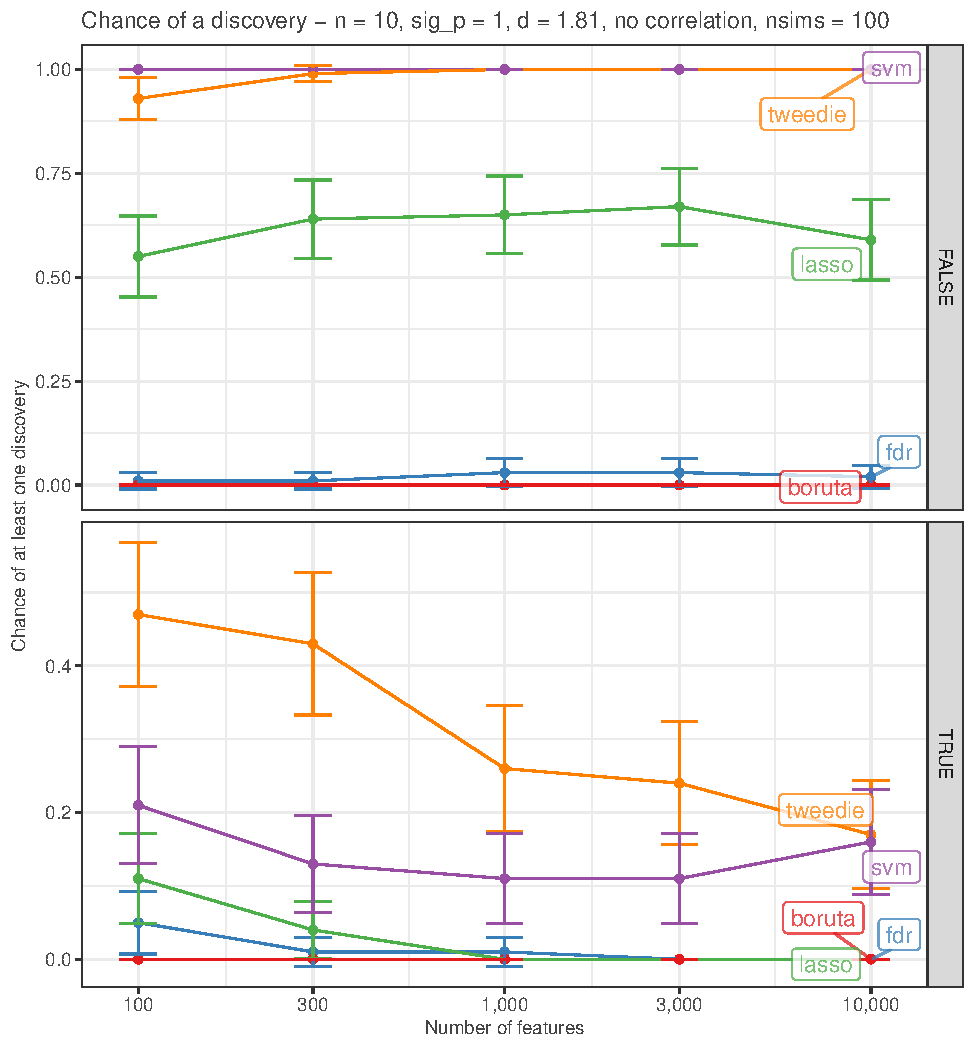
\includegraphics[width=0.49\linewidth]{main_files/figure-latex/unnamed-chunk-44-2} \end{center}

\begin{figure}

{\centering 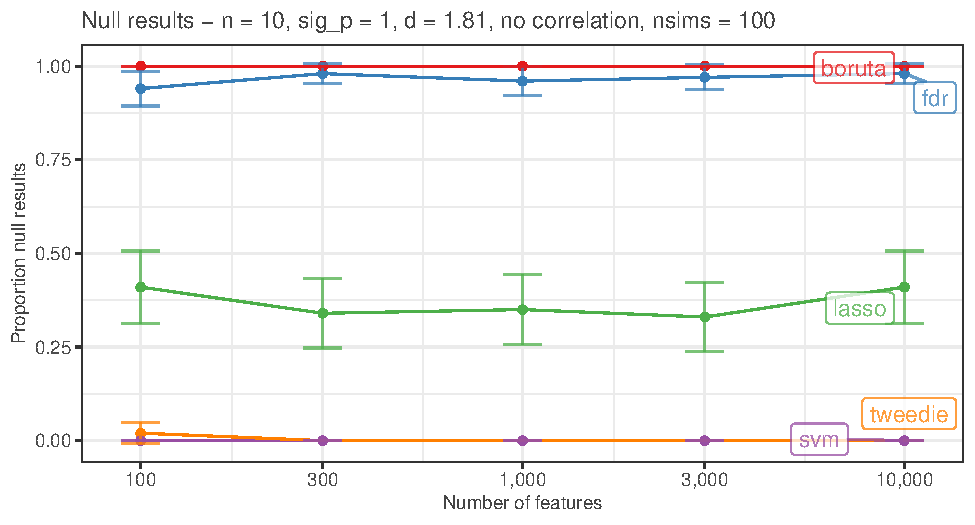
\includegraphics[width=0.49\linewidth]{main_files/figure-latex/B2-1} 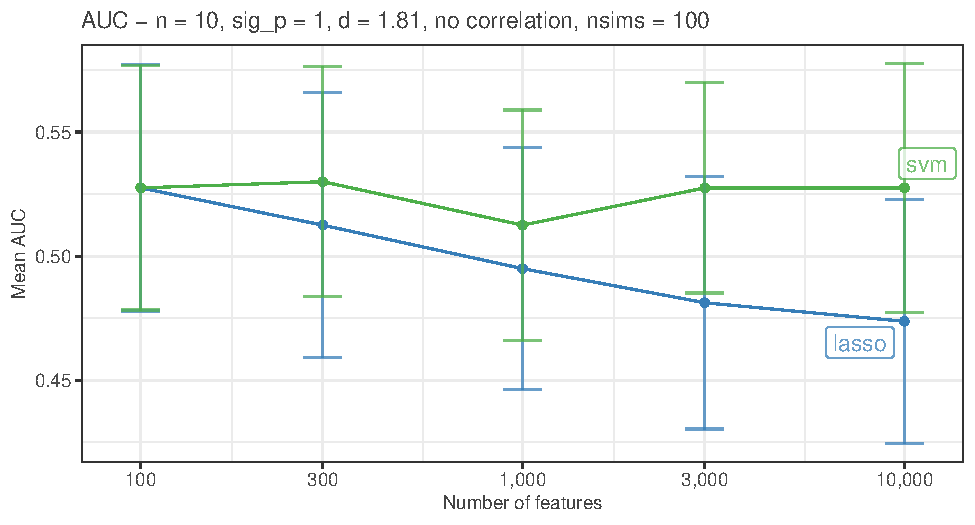
\includegraphics[width=0.49\linewidth]{main_files/figure-latex/B2-2} 

}

\caption{\textit{Upper left: Mean number of false and true discoveries for various numbers of features for every method. Upper right: Chance of at least one false and true discovery for various numbers of features for every method. Bottom left: Proportion of null results for various numbers of features for every method. Bottom right: Mean AUC of models built on selections by the model based methods for various numbers of features. 95\% confidence intervals are shown. In the case an interval is lacking, this has to do with the log scale of some of the plots.}}\label{fig:B2}
\end{figure}

\hypertarget{scenarios-c---in-between}{%
\subsection{Scenarios C - In between}\label{scenarios-c---in-between}}

Whereas the scenarios `A' and `B' were both extremes in the `optimistic-pessimistic-spectrum,' the scenarios `C' are somewhat in between with 30 samples and 3 significant features. There are no correlations between features. Within this setting, 2 different effect sizes are considered.

\hypertarget{scenario-c1}{%
\subsubsection{Scenario C1}\label{scenario-c1}}

This scenario has a relatively moderate effect size (0.95, or AUC = 0.75) per feature and reflects relatively poor conditions in this `in between' setting. The results can be seen in figure \ref{fig:C1}.

In terms of mean number of discoveries we see that SVM has the most false and true discoveries. FDR has the least both false and true discoveries. Tweedie and LASSO are able to keep the number of false discoveries relatively under control, that is more or less 3 throughout the range of p.~Boruta has increasingly more false discoveries and ever less true discoveries with growing p.~The same pattern is visible in terms of chances of at least one discovery. SVM is the only method that has a chance for at least one true discovery of more than 0.5 (0.57, SE 0.05) for p = 10,000. Tweedie comes in second at 0.28 (SE 0.04). These results indicate that this condition may be a boundary condition.

In terms of null results FDR is the worst method and SVM and Boruta the best methods. Tweedie has only a moderate amount of null results when p is larger than 300.

The AUC of the model based methods on the test set all behave in the same way. That is small values for AUC (around 0.6) for the smallest value for p and from there on decreasing with no distinction from 0.5 at p = 3,000 and more.

\begin{center}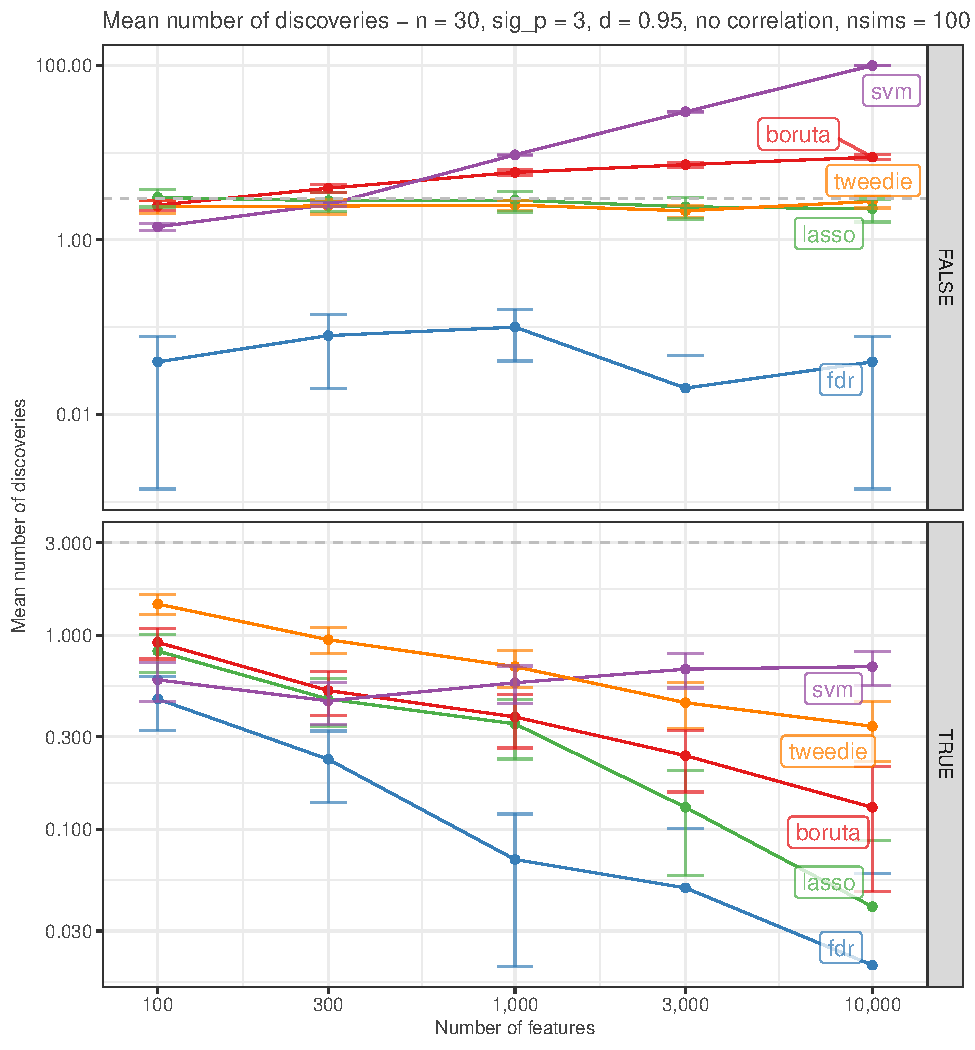
\includegraphics[width=0.49\linewidth]{main_files/figure-latex/unnamed-chunk-45-1} 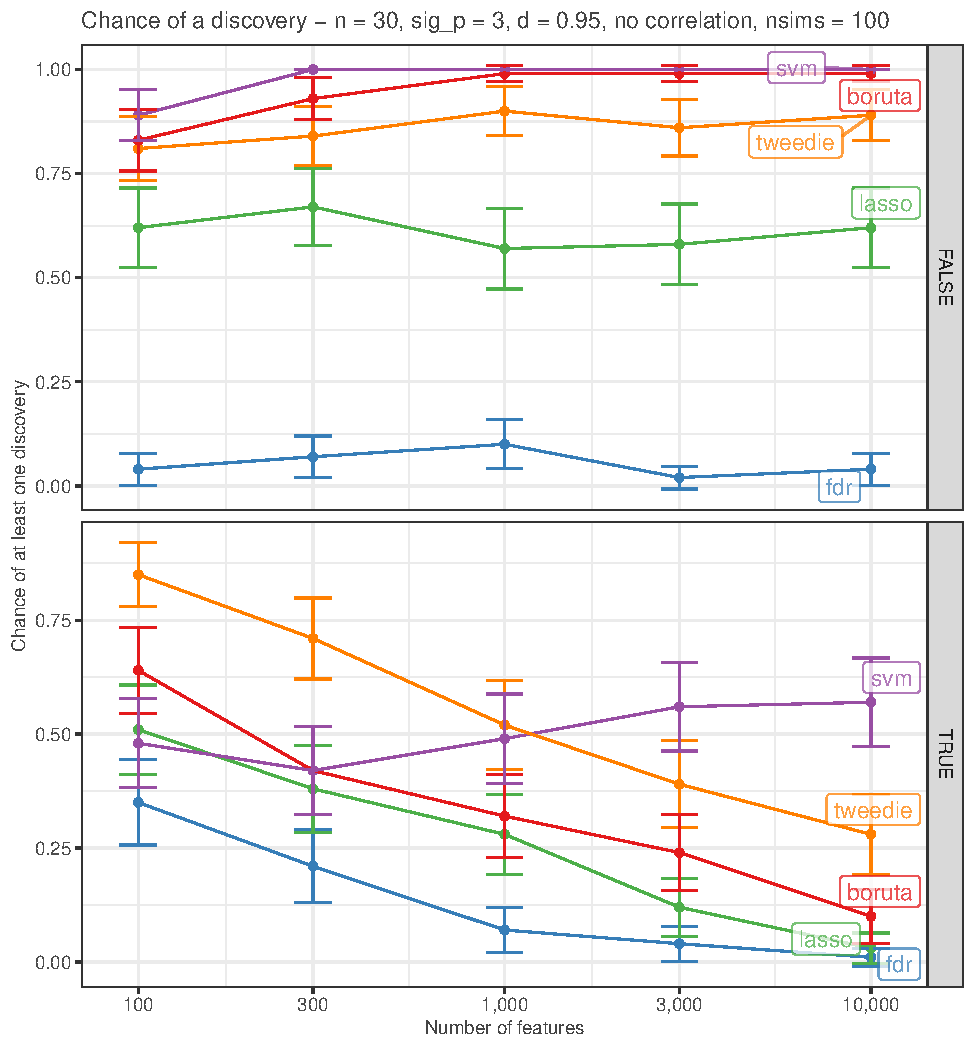
\includegraphics[width=0.49\linewidth]{main_files/figure-latex/unnamed-chunk-45-2} \end{center}

\begin{figure}

{\centering 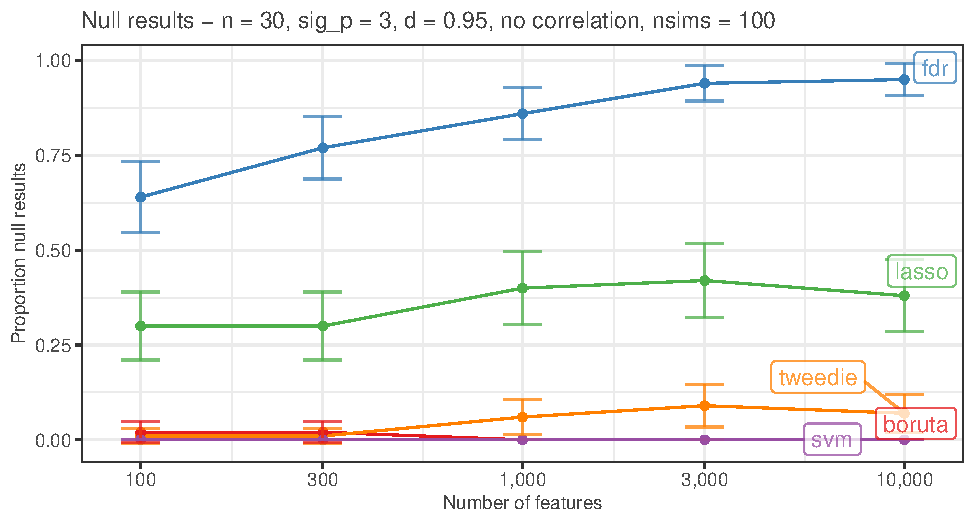
\includegraphics[width=0.49\linewidth]{main_files/figure-latex/C1-1} 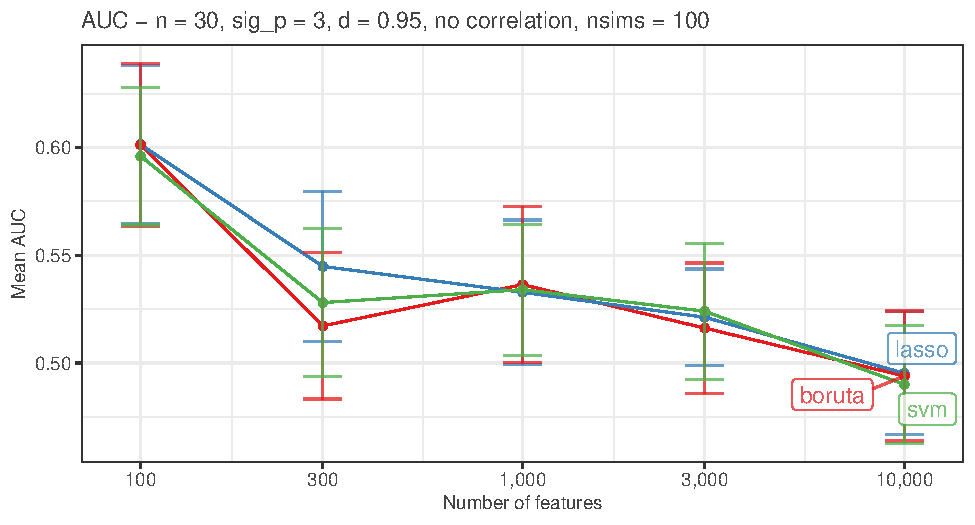
\includegraphics[width=0.49\linewidth]{main_files/figure-latex/C1-2} 

}

\caption{\textit{Upper left: Mean number of false and true discoveries for various numbers of features for every method. Upper right: Chance of at least one false and true discovery for various numbers of features for every method. Bottom left: Proportion of null results for various numbers of features for every method. Bottom right: Mean AUC of models built on selections by the model based methods for various numbers of features. 95\% confidence intervals are shown. In the case an interval is lacking, this has to do with the log scale of some of the plots.}}\label{fig:C1}
\end{figure}

\hypertarget{scenario-c2}{%
\subsubsection{Scenario C2}\label{scenario-c2}}

This scenario has a relatively larger effect size (1.3, or AUC = 0.82 per feature) and reflects somewhat better conditions than in scenario C1. The results can be seen in figure \ref{fig:C2}.

In terms of mean number of discoveries wee see that SVM has the most false and true discoveries. FDR has the lowest mean number of false and true discoveries. As the second best method, Tweedie has a mean number of true discoveries of 0.94 (SE 0.09) for p = 10,000. In terms of chance of at least one false discovery, Boruta and SVM are the worst performing methods while FDR is the best method. In terms of chance of at least one true discovery FDR and LASSO are the worst performing methods and Tweedie and SVM the best performing methods.

In terms of null results FDR is again the worst performing method while SVM, Boruta and Tweedie are the best performing methods.

The AUC measured on the test set for the model based methods was highest for LASSO, except at p =10,000 where all methods perform equally poor.

\begin{center}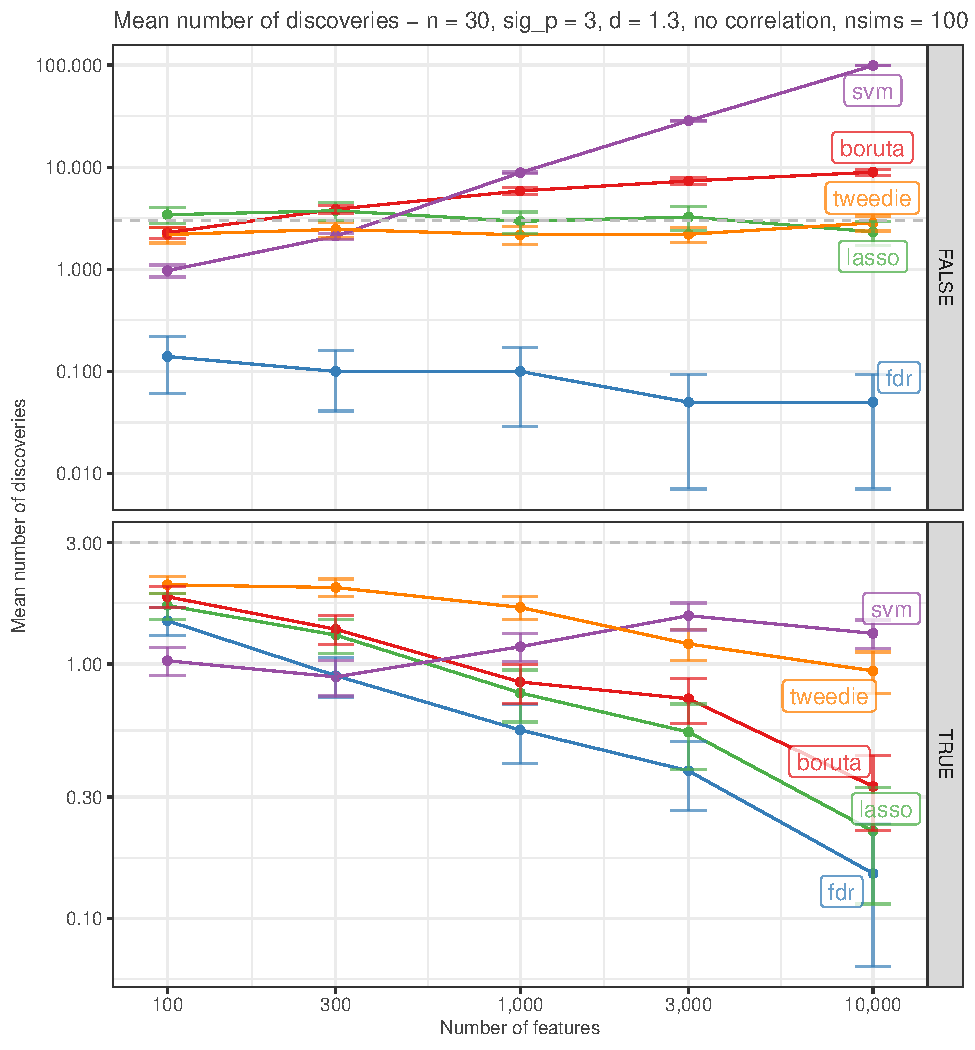
\includegraphics[width=0.49\linewidth]{main_files/figure-latex/unnamed-chunk-46-1} 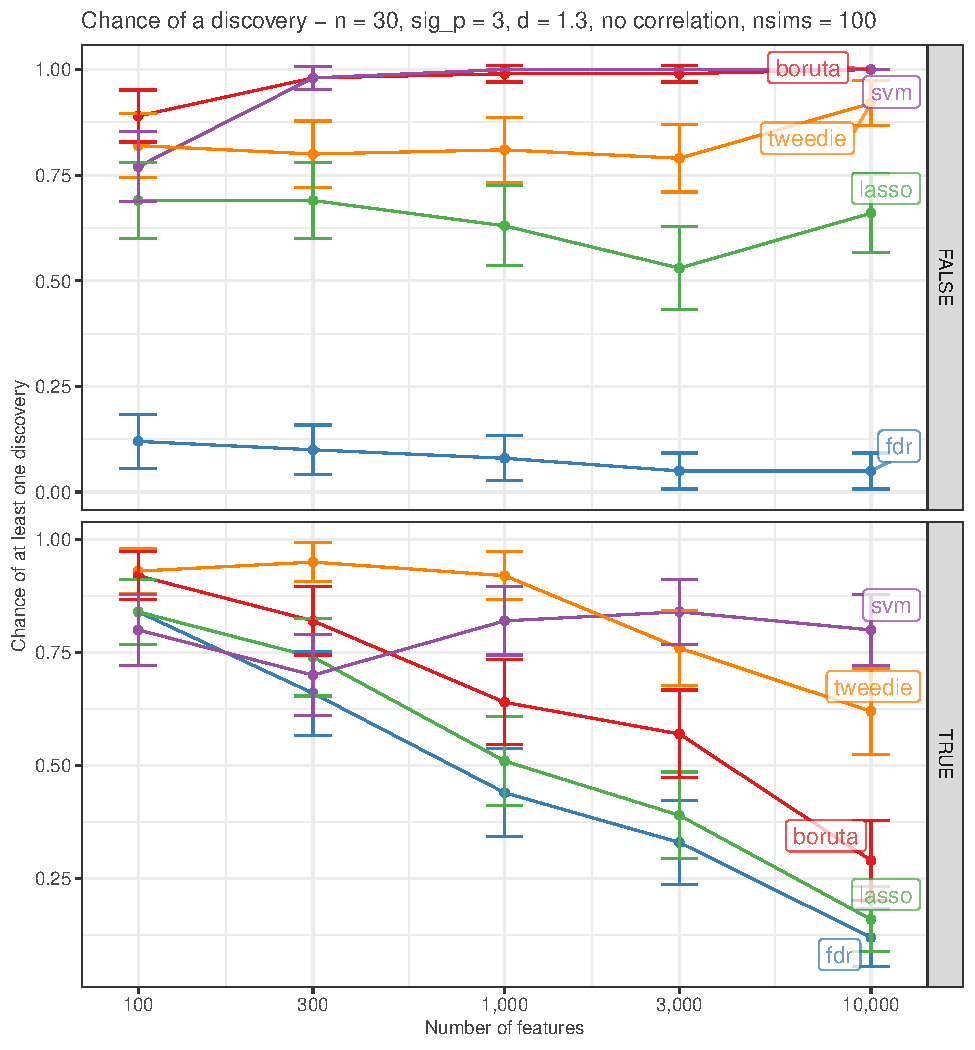
\includegraphics[width=0.49\linewidth]{main_files/figure-latex/unnamed-chunk-46-2} \end{center}

\begin{figure}

{\centering 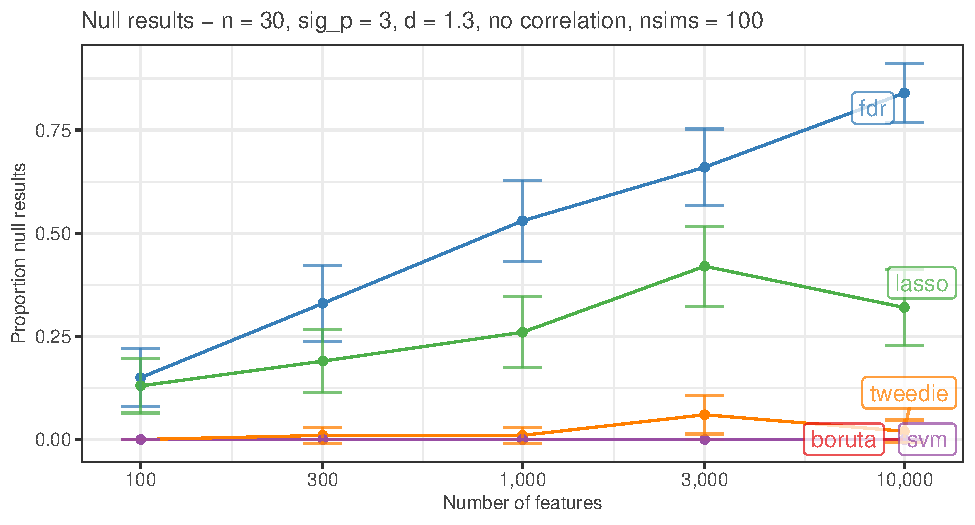
\includegraphics[width=0.49\linewidth]{main_files/figure-latex/C2-1} 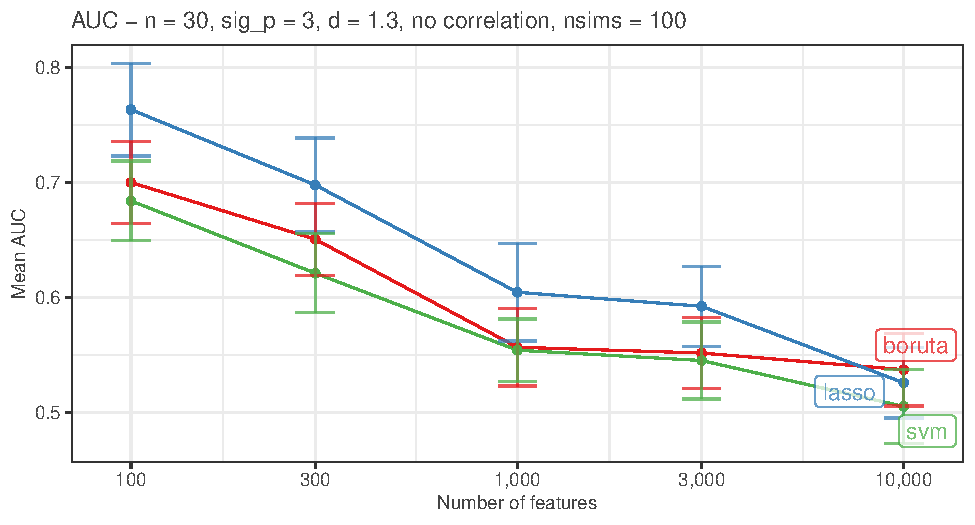
\includegraphics[width=0.49\linewidth]{main_files/figure-latex/C2-2} 

}

\caption{\textit{Upper left: Mean number of false and true discoveries for various numbers of features for every method. Upper right: Chance of at least one false and true discovery for various numbers of features for every method. Bottom left: Proportion of null results for various numbers of features for every method. Bottom right: Mean AUC of models built on selections by the model based methods for various numbers of features. 95\% confidence intervals are shown. In the case an interval is lacking, this has to do with the log scale of some of the plots.}}\label{fig:C2}
\end{figure}

\hypertarget{scenario-d}{%
\subsubsection{Scenario D}\label{scenario-d}}

This scenario is there to be able to evaluate the methods when there are no significant features. The number of samples is set at 20. The results can be seen in figure \ref{fig:D}.

In terms of number of false discoveries FDR is the best method throughout the entire range of p.~LASSO finds on average between 1 and 3 false discoveries and is stable across p.~Tweedie and Boruta are close to one another with on average between 3 and 10 false discoveries. Both methods perform wors with increasing number of features. SVM always picks the top 1\%, so there will be 1\% of p false discoveries. More or less the same conclusions can be drawn from the chances of at least one false discovery plot.

\begin{figure}

{\centering 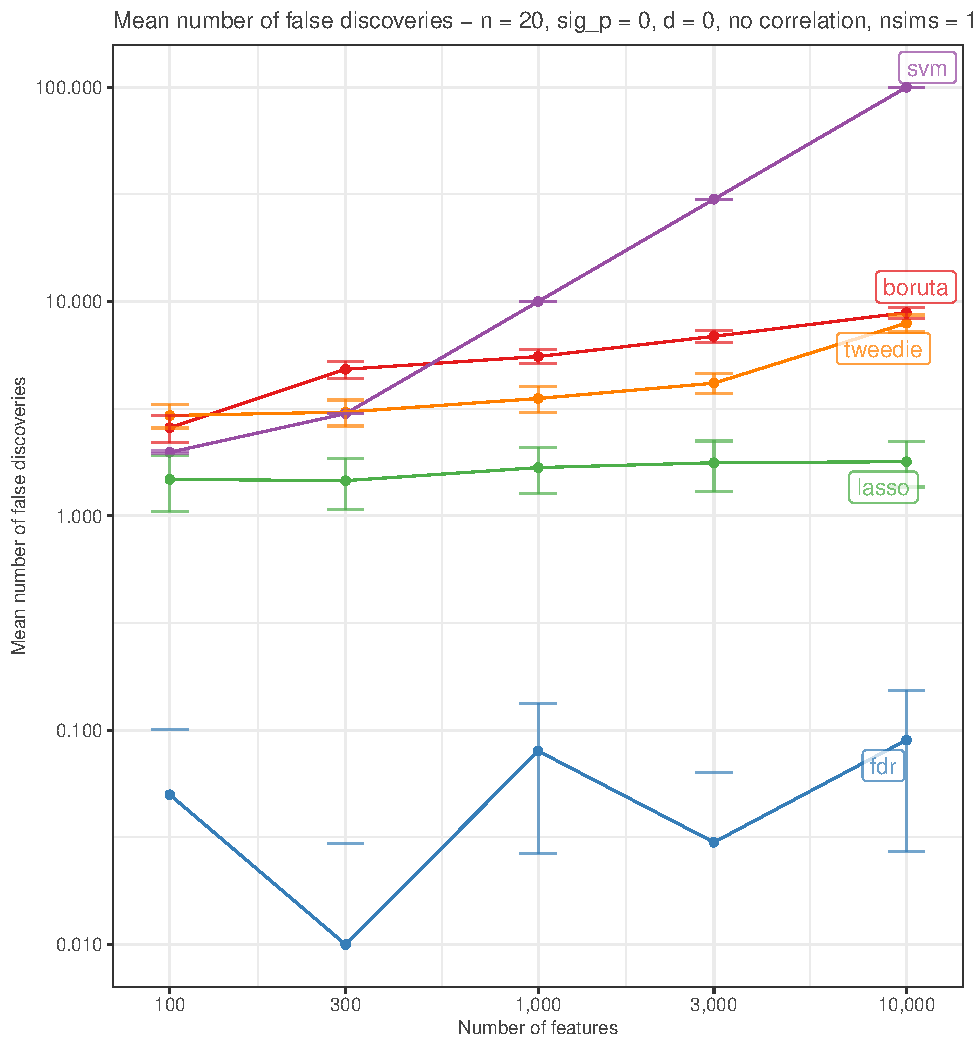
\includegraphics[width=0.49\linewidth]{main_files/figure-latex/D-1} 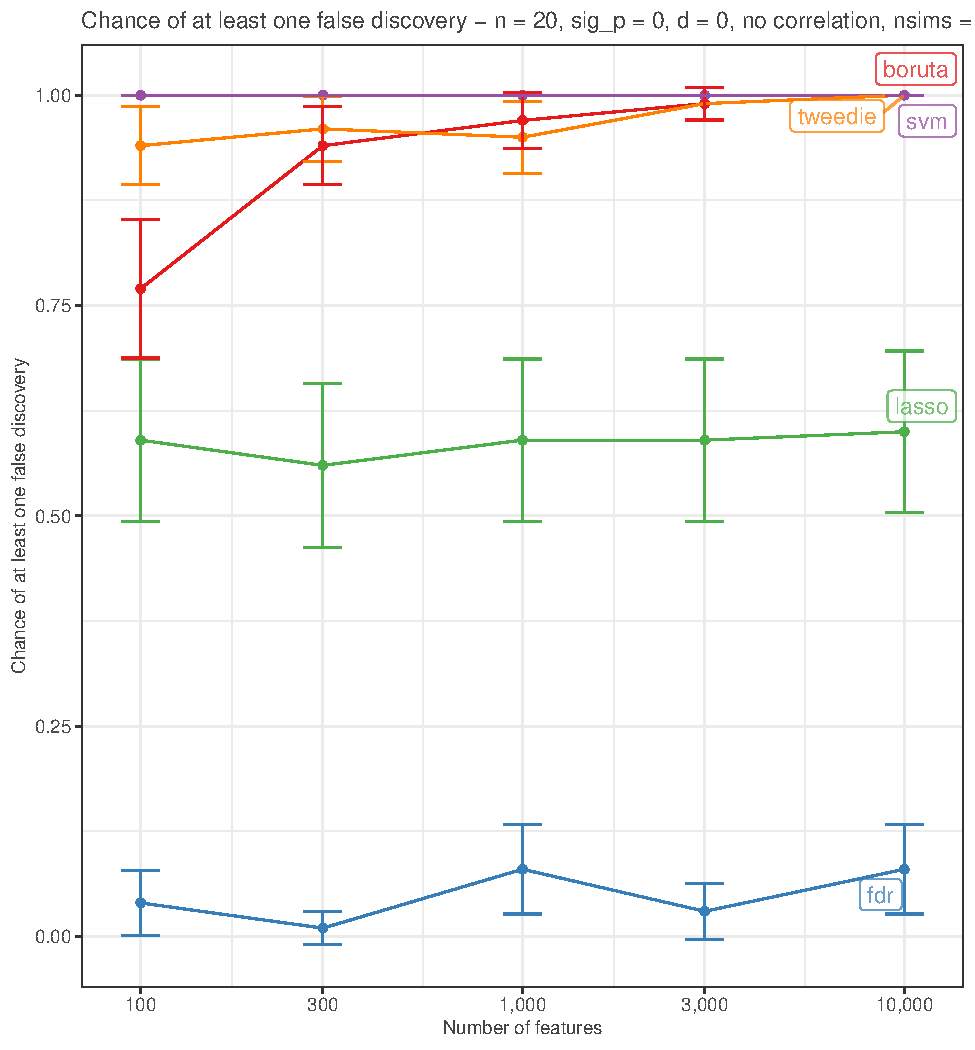
\includegraphics[width=0.49\linewidth]{main_files/figure-latex/D-2} 

}

\caption{\textit{Left: Mean number of false discoveries for various numbers of features for every method. Right: Chance of at least one false discovery for various numbers of features for every method.}}\label{fig:D}
\end{figure}

\hypertarget{block-correlation-structure-scenarios}{%
\subsection{Block correlation structure scenarios}\label{block-correlation-structure-scenarios}}

The most `forgiving' scenarios of scenarios A and C are selected and rerun with a block correlation structure in the data generating mechanism as described in the methods section. Only the most optimistic scenarios are selected because of the fact that we expect the performance to drop. In that way it is not very informative to try a condition with already very poor performances. This is also the reason why no scenario from the B scenarios is selected.

In these scenarios, data with at most 3,000 features were simulated because our system failed at p = 10,000.

\hypertarget{scenario-a1-with-block-correlation-structure}{%
\subsubsection{Scenario A1 with block correlation structure}\label{scenario-a1-with-block-correlation-structure}}

The results can be seen in figure \ref{fig:blockA1}.

In terms of mean number of false discoveries we see that Tweedie performs poorly at p = 100 and performs gradually better with growing number of features. At 3,000 features Tweedie is the second best performing method. LASSO performs more or less at the same level throughout the range of p.~Boruta is among the best performing methods at p = 100 but gradually becomes worse and ends with the second to highest mean number of false discoveries. SVM also starts off among the best performing methods at p = 100 and gradually worsens and ends as poorest performing method. FDR is the best performing method throughout the range of p.

In terms of mean number of true discoveries we see that Tweedie is consistently the best or among the best performing methods. The decline in performance of Tweedie with growing p seems to be the smallest (apart from SVM, which has an increasing performance), on the log scale. SVM is among the least performing methods with smaller numbers of features and gets better at p = 1,000 and is at the level of Tweedie at p = 3,000. FDR and Boruta show a similar pattern with Boruta showing a poorer performance than FDR. LASSO doesn't do well in these conditions. It consistently drops in performance throughout the range of p while it started already at the second to last place at p = 100.

In terms of chances of at least one false discovery we see more or less the same pattern as discussed above, with the exception that LASSO seems a bit more conservative than Tweedie, however, the differences are not always meaningful (e.g.~at p = 3,000 there is no difference). In terms of chances of at least one true discovery we see more or less the same pattern, except for FDR which performs worse than one would expect on the basis of the mean numbers of true discoveries and performs now worse than Boruta.

In terms of null results FDR is the worst performing method while Tweedie, SVM, and Boruta are the best performing methods. Of these, Tweedie has the most null results at higher numbers of features.

In terms of mean AUC we see that all models perform better than 0.5 for every value for p.~All values are close to each other with the only exception being p = 100, where LASSO performs better than the 2 other methods.

\begin{center}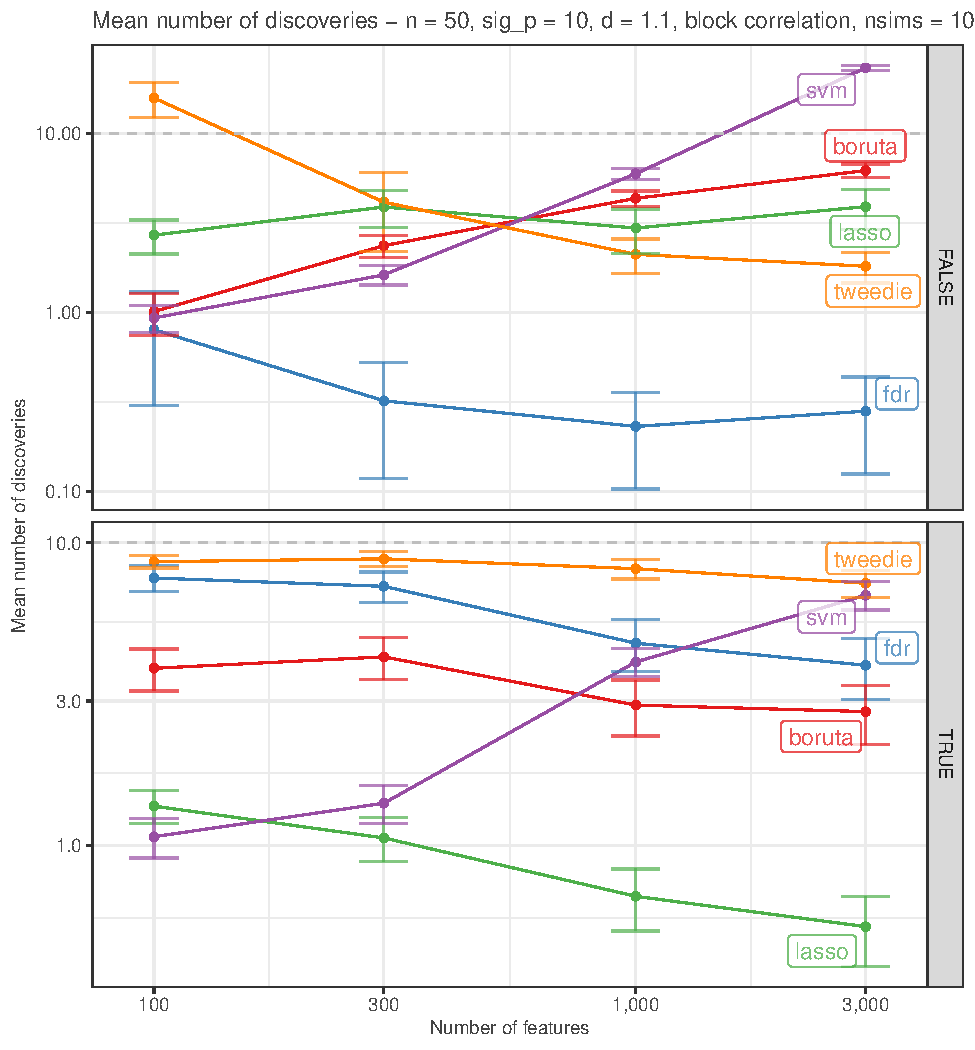
\includegraphics[width=0.49\linewidth]{main_files/figure-latex/unnamed-chunk-47-1} 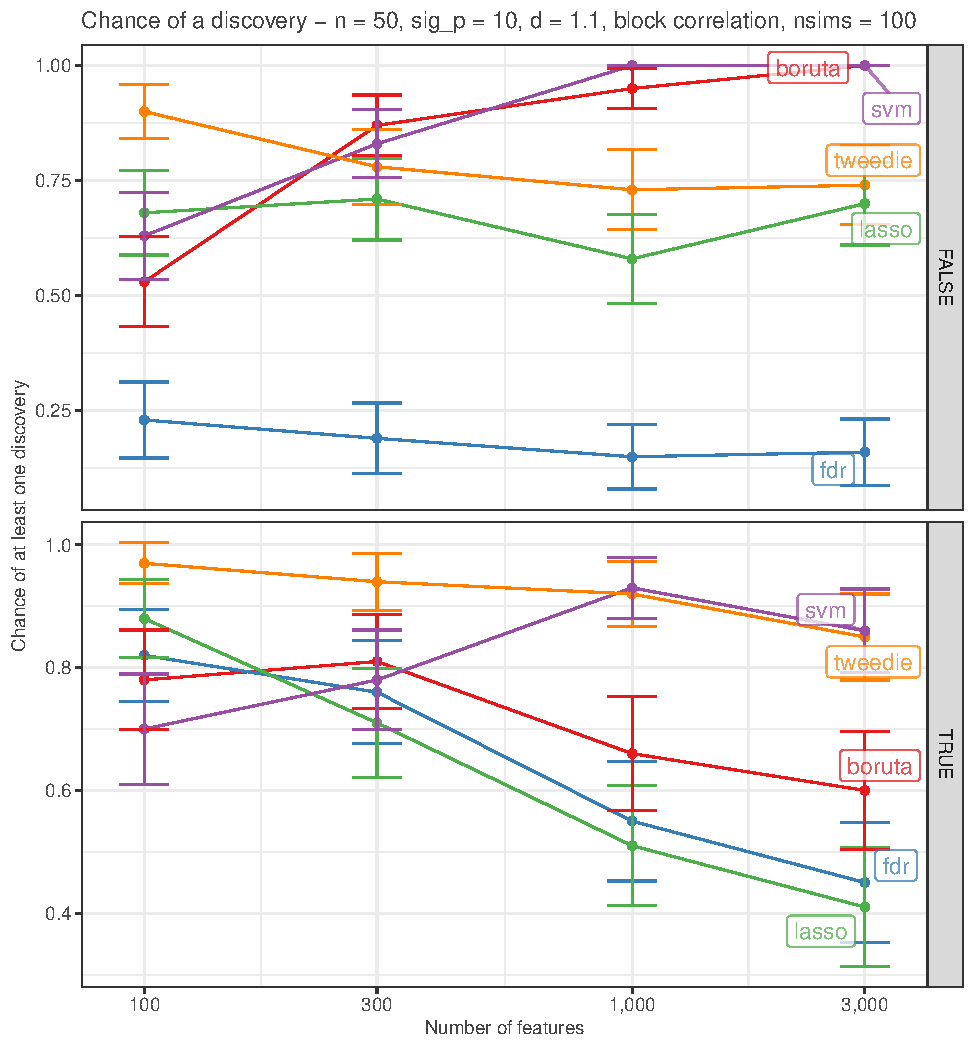
\includegraphics[width=0.49\linewidth]{main_files/figure-latex/unnamed-chunk-47-2} \end{center}

\begin{figure}

{\centering 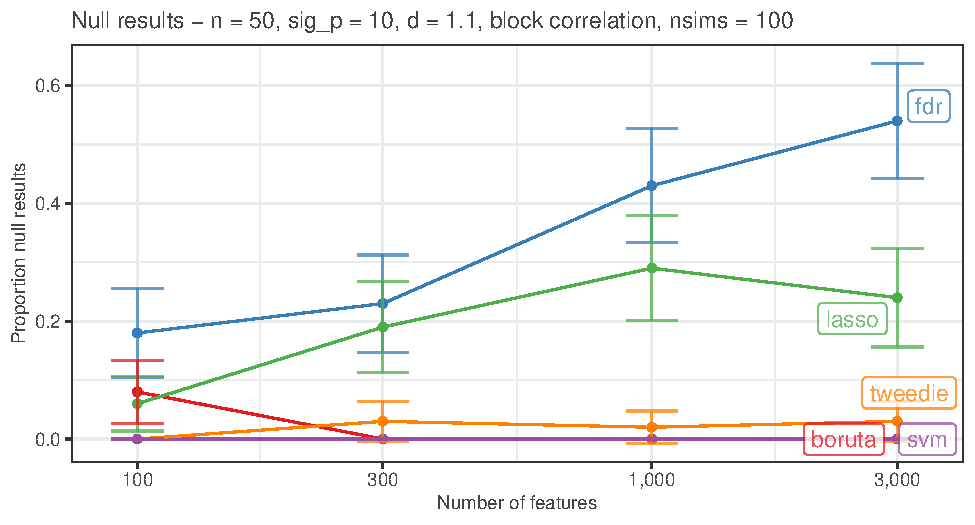
\includegraphics[width=0.49\linewidth]{main_files/figure-latex/blockA1-1} 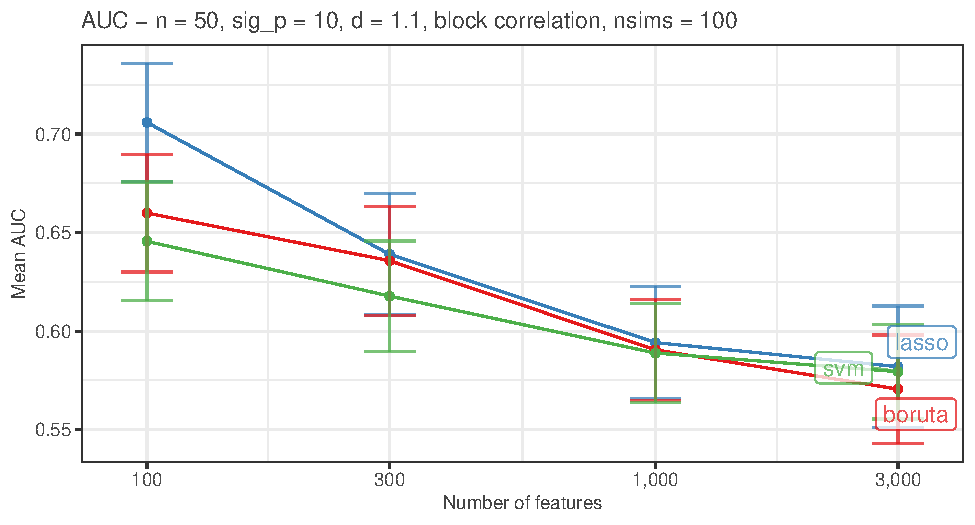
\includegraphics[width=0.49\linewidth]{main_files/figure-latex/blockA1-2} 

}

\caption{\textit{Upper left: Mean number of false and true discoveries for various numbers of features for every method. Upper right: Chance of at least one false and true discovery for various numbers of features for every method. Bottom left: Proportion of null results for various numbers of features for every method. Bottom right: Mean AUC of models built on selections by the model based methods for various numbers of features. 95\% confidence intervals are shown. In the case an interval is lacking, this has to do with the log scale of some of the plots.}}\label{fig:blockA1}
\end{figure}

\hypertarget{scenario-c2-with-block-correlation-structure}{%
\subsubsection{Scenario C2 with block correlation structure}\label{scenario-c2-with-block-correlation-structure}}

The results can be seen in figure \ref{fig:blockC2}.

In terms of mean number of false discoveries we see that SVM performs better than most methods at p = 100 and 300 and performs the poorest at p = 1,000 and p = 3,000. Boruta shows the same pattern as SVM, although much less pronounced. LASSO and Tweedie perform consistently at around 3 mean false discoveries, while FDR performs the best with very few discoveries on average (aroudn 0.3 to 0.1).

In terms of mean number of true discoveries we see that Tweedie is the best or among the best performing methods, except at p = 3,000 where SVM is slightly better. SVM performs among the poorest performing methods for relatively small values for p (100 and 300) and is among the best methods at higher values for p (1,000 and 3,000). After Tweedie, the best performing methods in order are Boruta, FDR, while LASSO comes in last.

In terms of chances of true/false discoveries we see more or less the same patterns. We see again that LASSO is a bit more conservative than Tweedie. In terms of true discveries we see that FDR and LASSO switched places compared to mean number of true disoveries.

In terms of null results FDR is the worst performing method while Tweedie, SVM, and Boruta are again the best performing methods. Of these, Tweedie has again the most null results at higher numbers of features.

In terms of mean AUC we see the same pattern of resutls as in A2 block correlated. All models perform better than 0.5 for every value for p.~All values are close to each other with the only exception being p = 100, where LASSO performs better than the 2 other methods.

\begin{center}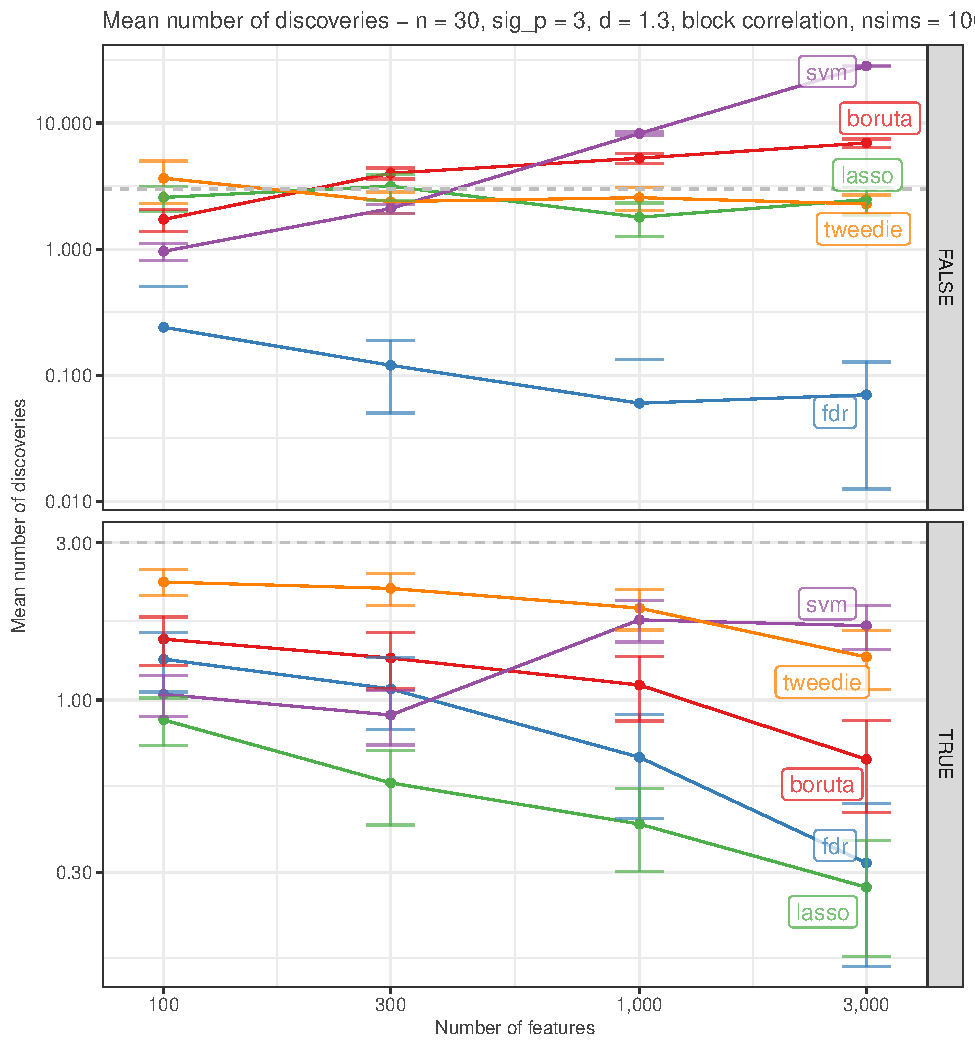
\includegraphics[width=0.49\linewidth]{main_files/figure-latex/unnamed-chunk-48-1} 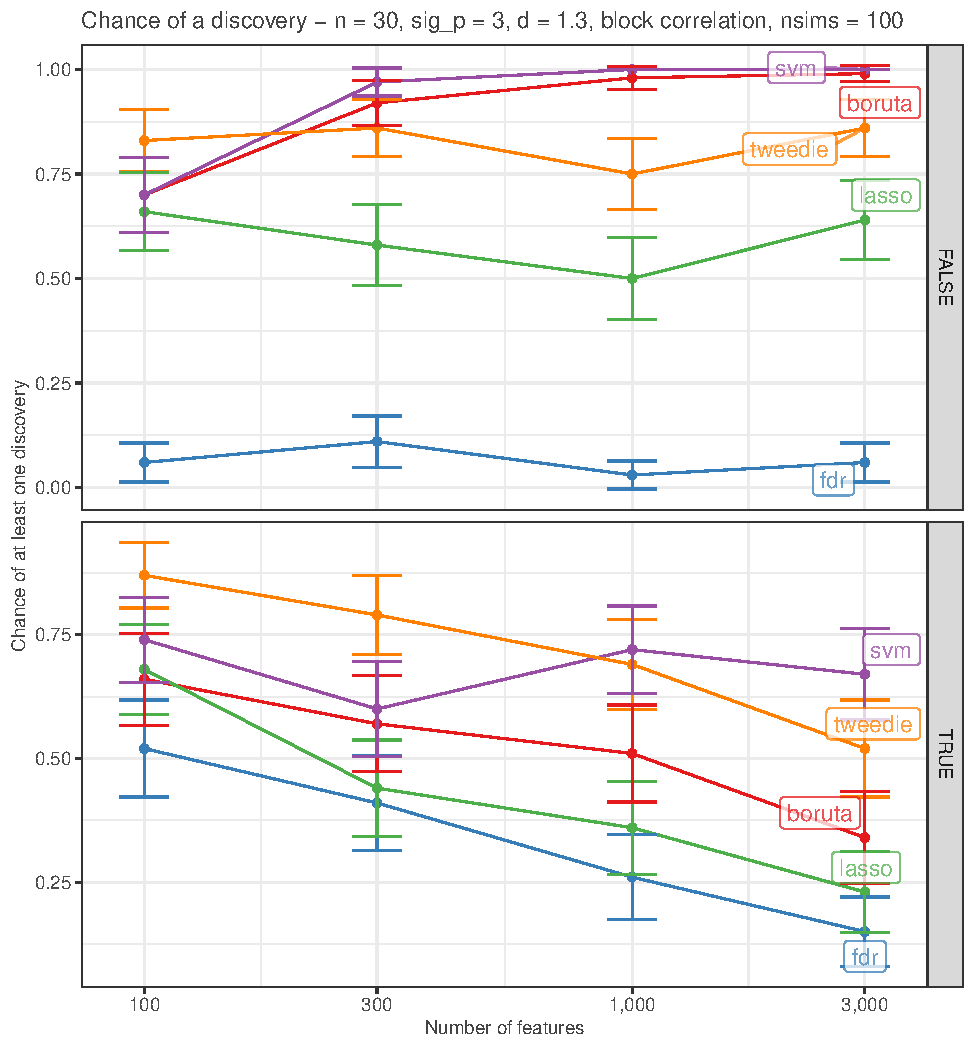
\includegraphics[width=0.49\linewidth]{main_files/figure-latex/unnamed-chunk-48-2} \end{center}

\begin{figure}

{\centering 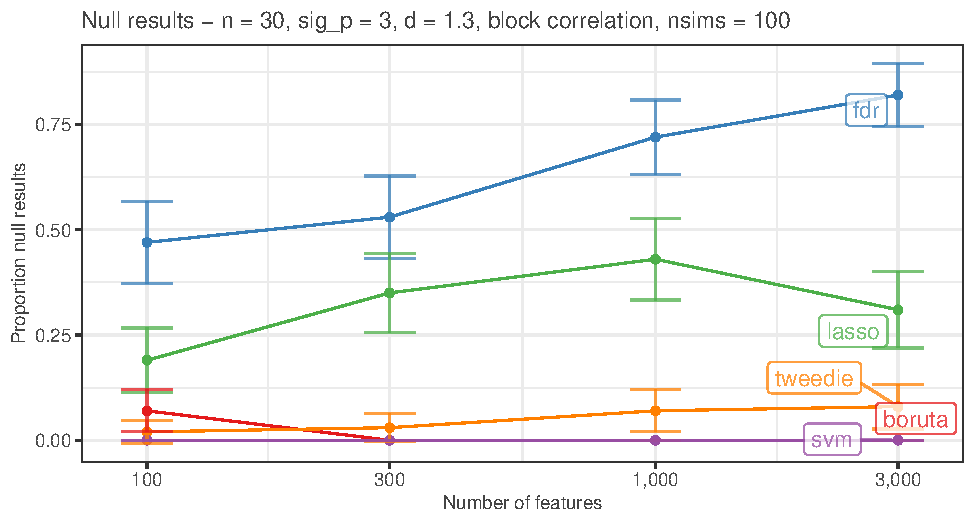
\includegraphics[width=0.49\linewidth]{main_files/figure-latex/blockC2-1} 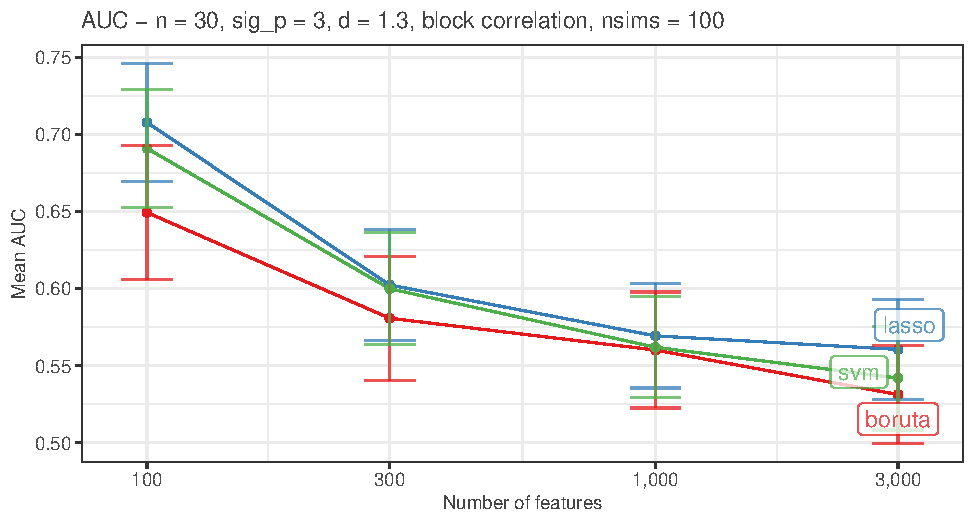
\includegraphics[width=0.49\linewidth]{main_files/figure-latex/blockC2-2} 

}

\caption{\textit{Upper left: Mean number of false and true discoveries for various numbers of features for every method. Upper right: Chance of at least one false and true discovery for various numbers of features for every method. Bottom left: Proportion of null results for various numbers of features for every method. Bottom right: Mean AUC of models built on selections by the model based methods for various numbers of features. 95\% confidence intervals are shown. In the case an interval is lacking, this has to do with the log scale of some of the plots.}}\label{fig:blockC2}
\end{figure}

\hypertarget{computation-time}{%
\subsection{Computation time}\label{computation-time}}

Although this not of primary concern for method users, it can be interesting too see how well methods scale with growing number of p with regard to computation time. The results can be seen in figure \ref{fig:timeresults}.

All computation times are relatively short which adds to the lack of concern regarding computation time from the perspective of method users. Though, we can see that Boruta seems to have difficulties with scaling. One could expect that if the number of samples and number of features keep increasing, the computation time might become an issue. Tweedie, on the other hand, seems to scale very well with growing number of features.

There is one additional result that draws the attention and that is that of SVM at p = 1,000 which is slower than at p = 3,000. The reason of this has to do with the halving of the features up to the point at which there are 250 or less features in the feature pool. At a starting point of 3,000 one ends up at 188 before the procedure starts to eliminate one feature at a time. At a starting point of 1,000 this is 250, which is higher and that is why the analysis takes longer on average.

\begin{figure}

{\centering 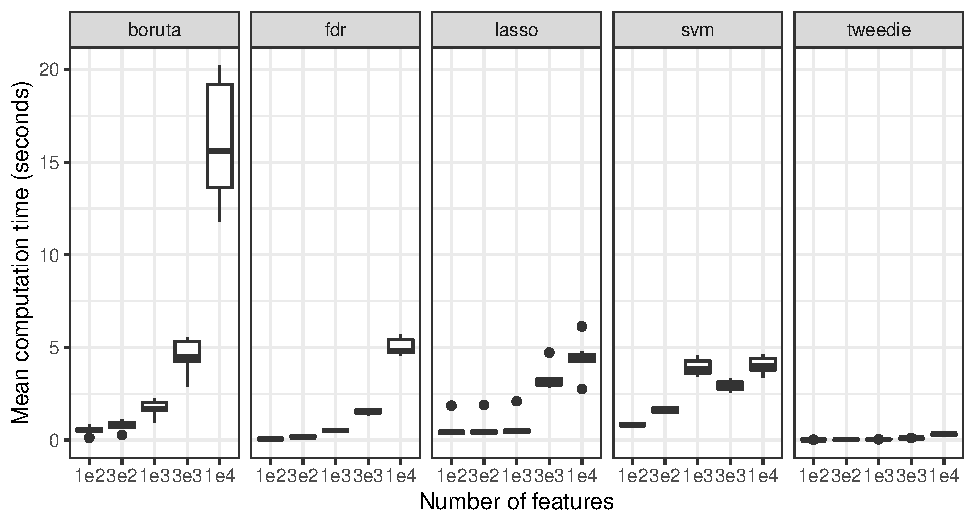
\includegraphics[width=1\linewidth]{main_files/figure-latex/timeresults-1} 

}

\caption{\textit{Boxplots of computation time for every method and for every number of features, across all simulations}}\label{fig:timeresults}
\end{figure}

\newpage

\hypertarget{discussion}{%
\section{Discussion}\label{discussion}}

\hypertarget{boundary-conditions}{%
\subsection{Boundary conditions}\label{boundary-conditions}}

From the results of scenario A3 we learn that at n = 50, and sig\_p = 10, d = 0.3 and at p larger than or equal to 1,000 virtually no method can deliver any satisfying results anymore. None of the methods have an expected number of true discoveries larger than 1 and this for the entire range of p.~None of the methods have a chance of having a true discovery below 0.4 (except at p = 100), while for all methods except FDR the chance of at least one false discovery is above 0.5 for the entire range of p.

The same is true for the B scenarios, that is no satisfying performance, where n = 10 and sig\_p = 1 for the entire range of p and both values for d.~In these scenarios the Boruta method totally failed to work. The other methods delivered very poor performances. Except for FDR (and Boruta, see above), all other methods had a chance of having at least one false discovery of above 0.5 for the entire range of p while the chance of having at least one true discovery was below 0.25 for the entire range of p in when d = 0.9. Performances were slightly better at a high effect size per feature. However they were still far beneath satisfactory levels.

In scenario C1 with n = 30, sig\_p = 3, d = 0.95 there were also very poor results when p was larger than or equal to 1,000. In terms of mean number of true discoveries only Tweedie was able to find on average more than one true discovery at p = 100, on average 1 true discovery at p = 300. From p = 1,000 on the mean number of true discoveries was less than 1 for every method while the mean number of false discoveries was larger than 1, except for FDR.

The conditions discussed above are what we call boundary conditions in which it is to be expected to have no or very few useful results in general. With in general, we mean that it is the case for all methods.

\hypertarget{formulation-of-guidelines}{%
\subsection{Formulation of guidelines}\label{formulation-of-guidelines}}

There is no one method that is best at everything, so what method to choose will depend on what is important to the problem at hand. If one values conservativeness more, then it is clear that FDR is the best choice. In all scenarios FDR was the best performing method with respect to keeping the number of false discoveries within reasonable limits. The method to avoid is the SVM. Because of the top 1\% rule, it always picks 100 features at p = 10,000. In this way there will be a lot of false discoveries when sig\_p is rather small. The same conclusion can be made on the basis of the results regarding the chance of at least one false discovery. This is not that surprising. Another method to avoid when striving for conservativeness is Boruta as it performed poorly with regard to the chance of at least one false discovery in scenarios A (optimistic), C (in between), D (no sig\_p) and both block correlation scenarios. In the B scenarios (pessimistic) Tweedie was also among the least conservative methods.

If one, on the other hand, values many true discoveries at the cost of more false discoveries, then other methods are in place. SVM is almost consistently among the best performing methods in this regard. Only in A1block (optimistic, large effect size), did SVM fail to be among the best methods. The downside of SVM is of course a high number of false discoveries. Other methods that deliver good results in terms of number of true discoveries is Tweedie (A1, B, C2, A1block, C2block). Most often, Tweedie is less `aggressive' than SVM in that it doesn't result in that much false discoveries as SVM does. It is interesting that Tweedie is present in the list of well performing methods in the block correlation scenarios while SVM is not in both. This could perhaps indicate that Tweedie is better suited when the data gets more realistic properties.

Methods to avoid in this regard are FDR and LASSO. FDR is consistently among the worst methods. This is not surprising since it is the most conservative method (see above). LASSO didn't do well in this regard in scenarios A1, B1, C2, A1block, and C2block. It is interesting to see that LASSO was among the worst performing methods in the block correlation scenarios. The fact that it has difficulties in dealing with highly correlated features is a well known weakness of the LASSO. Highly correlated features are a problem for coefficient estimation. In such cases multicollinearity, the presence of highly intercorrelated features, results in highly variable estimates. The LASSO can deal with these kinds of features by removing all but one. However, the method is agnostic of which feature is a true or false feature. Thus, in highly correlated situations the lasso will discard many correlated features. And it does so unknowingly of feature status (true or false).

This downside of the LASSO has also a benefit. Getting rid of multicollinearity by setting some coefficients to zero will benefit prediction. When prediction is of main interest, the LASSO is often the better choice compared to the other model based methods. It was the best method in scenarios A1 (optimistic, relatively large effect size), A3 (optimistic, yet small effect size), C2 (in between, larger effect size), A1block, and C2block. SVM performed best in scenarios A2 and C2block. As such Boruta is often to be avoided.

If one really wants to avoid null results, then one thing to consider is using SVM. SVM will always produce results because of the top 1\% rule. The added benefit is that we have seen that SVM is often good at capturing the significant features. Yet, it comes with the cost of a lot of false discoveries as well. Other methods to consider are Tweedie (A1, B1, B2, C2) and Boruta (A1, A2, A3, C1, C2, A1block, and C2block). However, Boruta did not perform very well with regard to other measures.

All in all, the results of Tweedie look promising because the method often performs quite well with regard to true discoveries and `not so bad' with regard to false discoveries. It is not possible to have a method that is optimal in both. Yet, Tweedie seems to find some sort of middle ground in many scenarios.

One other thing to consider is the ease of use. While the application of Tweedie's formula is in essence not that complicated, it is a fact that no off-the-shelf implementation is available. This can and will be an obstacle for some, if not many, people. Maybe such a solution could become available in the future, for example in the form of an R-package.

\hypertarget{limitations-of-the-current-study}{%
\subsection{Limitations of the current study}\label{limitations-of-the-current-study}}

In the current study a lot of simulation parameters were manipulated: number of features, number of significant features, sample size, effect size per feature, correlation structure. Because there were so many parameters it was impossible to implement a full factorial design in which all combinations of values are explored. In this study, only a tiny fraction of the entire simulation parameter space was explored. We chose not to use a full factorial design because it would sooner rather than later become practically unfeasible to do the entire simulation study.

Yet, it might be that a full factorial design with a tighter focus would be feasible and interesting. Now we chose to entangle number of samples with number of significant features and compose them together as optimistic, pessimistic and in between. While this was a means to keep things workable, it leaves the question what the effect is of the one or the other. Which of the 2 is more important in terms of boundary conditions? Maybe the disentanglement of sample size and number of significant features could lead to other guidelines.

Even with the current entanglement, it is still the case that we only explored a tiny fraction of that subspace of the simulation parameter space. And it may be that we did not choose the most interesting values. The exploratory simulations were intended to mitigate this somewhat, but the problem isn't solved by that. The problem is only shifted.

Another possible remark are the included methods. In ideal circumstances one would include all the most relevant methods. However, this is practically not possible. In this study there were 2 classes of methods: methods that involve hypothesis tests and feature selection methods that are based on prediction models. As we have seen, not all performance measures are applicable to every method, which is not ideal.

An other weakness is the simplicity of the data generating mechanism. Simple data generating mechanisms allow for easy interpretation. On the other hand, it could be that because of that simplicity the results aren't applicable to real analyses. Methods like SPsimSeq (Assefa, Vandesompele, and Thas 2020) could be used to enhance the realism of the simulated data and as a consequence also enhance the applicability of the results.

A last thing to consider is the difference in parameter tuning of the LASSO in comparison with SVM and Boruta. Although both SVM and Boruta have hyperparameters that can be tuned, we only used the default values.

\newpage

\hypertarget{example-analysis}{%
\section{Example analysis}\label{example-analysis}}

In this last section we will perform an example analysis. The data that we will use come from Hung, Baldi, and Hatfield (2002) and found it via the userguide of the limma bioconductor package. In this user guide there is example code given that allows one to set up the data. This example code was used only to import and set up the data so that it was in a format that was familiar.

Hung, Baldi, and Hatfield (2002) explain that

\begin{quote}
the purpose of the work presented here is to identify the network of genes that are differentially regulated by the global E. coli regulatory protein, leucine-responsive regulatory protein (Lrp), during steady state growth in a glucose supplemented minimal salts medium. Lrp is a DNA-binding protein that has been reported to affect the expression of approximately 55 genes.
\end{quote}

We will approach the data only from a statistical point of view.

\hypertarget{data-set-description-and-exploratory-analysis}{%
\subsection{Data set description and exploratory analysis}\label{data-set-description-and-exploratory-analysis}}

This dataset consists of 7312 features measured on 8 samples. There are 2 classes, each with 4 samples. Mean, standard deviation, median, inter quartile range (iqr), minimum (min), and maximum (max) was calculated for every gene and strain combination. This allows to visualize the distributions of these statistics across genes for every strain. This visualization can be seen in figure \ref{fig:descriptives}. The distributions of the statistics of the 2 strains look very alike. There is a small difference noticable in the distribution of standard deviation and inter quartile range, meaning that expression levels of lrp- are slightly more variable than expression levels of lrp+.

\begin{figure}

{\centering 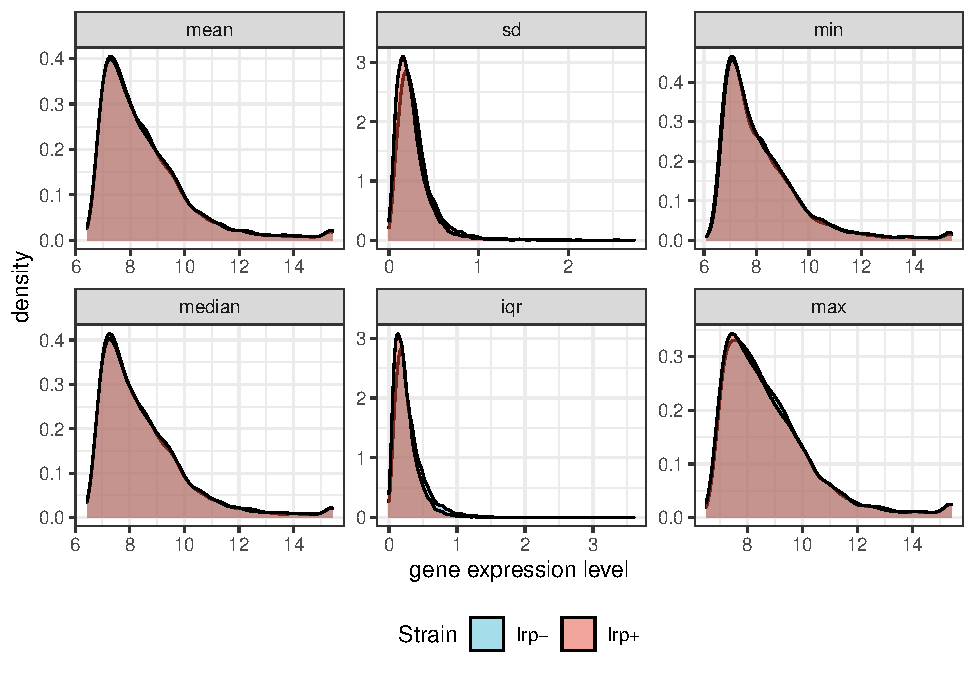
\includegraphics[width=0.75\linewidth]{main_files/figure-latex/descriptives-1} 

}

\caption{\textit{Distributions of descriptive statistics of gene expression levels of both strains.}}\label{fig:descriptives}
\end{figure}

\hypertarget{application-of-tweedies-formula}{%
\subsection{Application of Tweedie's formula}\label{application-of-tweedies-formula}}

For this analysis, we will use Tweedie as method. This is because Tweedie performed best in the more realistic scenarios (block correlation). Also, there is little data at hand, only 8 samples. In order to make the most use out of the data it makes more sense to use all data for t-tests than to split the data in a training and test set like we would when using model based methods.

Because FDR is far too concervative and we don't want to risk missing potential biomarkers we opt for Tweedie.

In order to find out which genes are differentially expressed between strains the following null hypotheses were tested against the following alternative hypotheses:

\[\left.\begin{aligned} H_{0i}: \mu_{lrp- i} = \mu_{lrp+i} \\ H_{ai}: \mu_{lrp- i}\neq \mu_{lrp+i} \end{aligned} \right \} \space  \space i = \{1,\dots,7312\} \]

In these hypotheses, \(\mu_{lrp-i}\) and \(\mu_{lrp+i}\) are the population means of the gene expression level of the ith gene in the lrp- and lrp+ strain respectively.

After the t-tests are performed, a histogram of the test statistics is constructed. The middle of each bin and the counts are used to perform a 4th degree polynomial poisson regression (log link). The coefficients can be found in table \ref{tab:coef}

\begin{figure}

{\centering 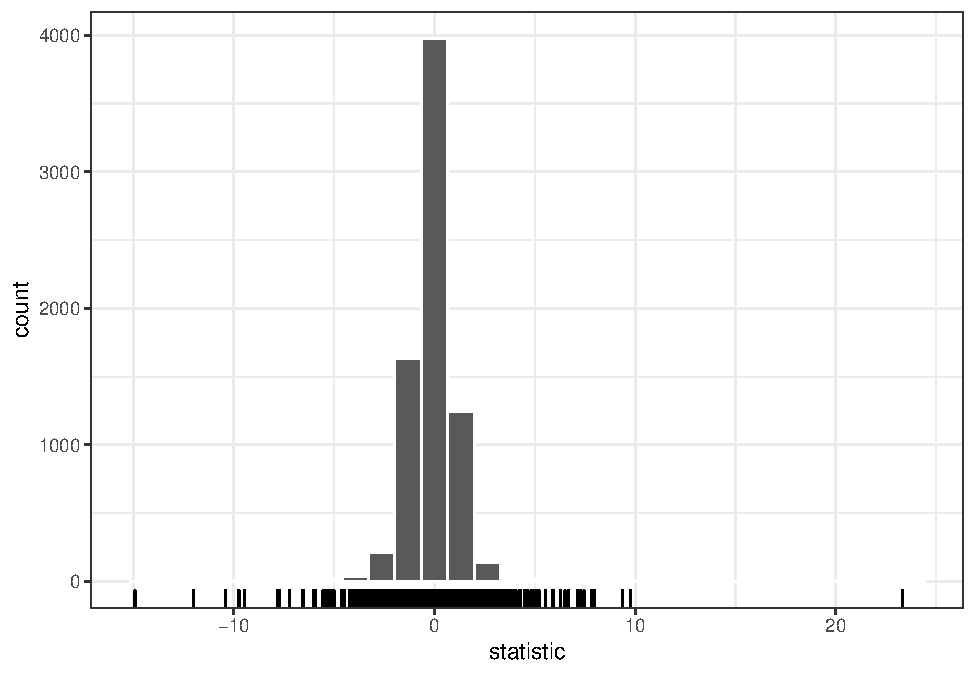
\includegraphics[width=0.75\linewidth]{main_files/figure-latex/hist-1} 

}

\caption{\textit{Histogram of the test statistics. The vertical dashes show the individual data points.}}\label{fig:hist}
\end{figure}

\begin{table}

\caption{\label{tab:coef}Coefficients of 4th degree polynomial poisson regression on bin counts.}
\centering
\begin{tabular}[t]{lr}
\toprule
Coefficient & value\\
\midrule
Intercept & 8.0740841\\
Poly 1 & -0.0440204\\
Poly 2 & -0.3814665\\
Poly 3 & -0.0083491\\
Poly 4 & 0.0010862\\
\bottomrule
\end{tabular}
\end{table}

After the log derivative and the variance of the test statistics is estimated we perform the correction. Figure \ref{fig:beforeafter} shows the curve of corrected test statistic vs.~uncorrected test statistic.

\begin{figure}

{\centering 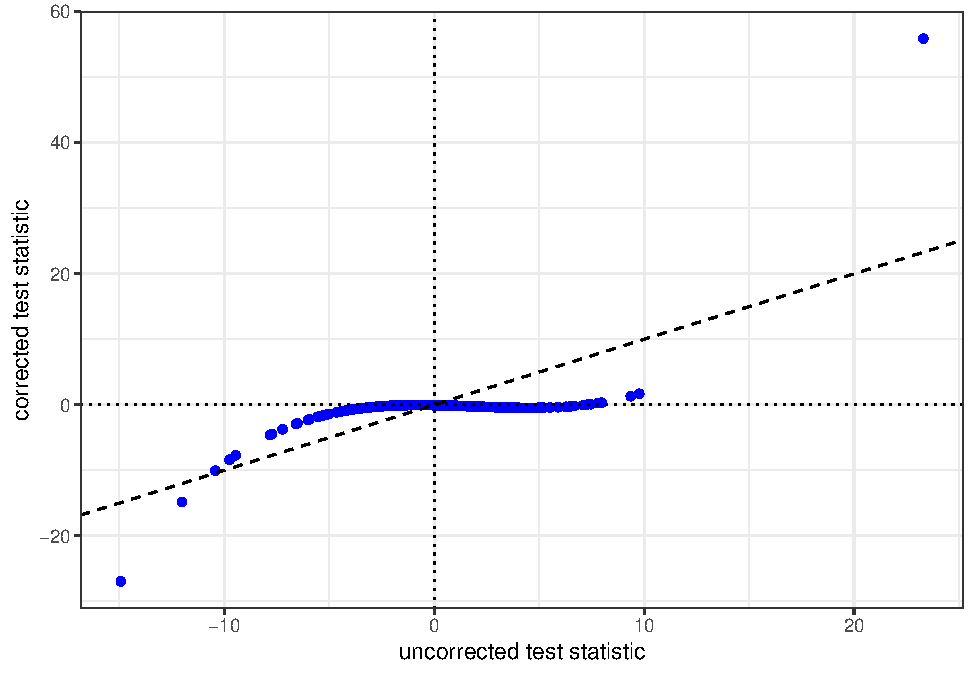
\includegraphics[width=0.75\linewidth]{main_files/figure-latex/beforeafter-1} 

}

\caption{\textit{Corrected vs. uncorrected test statistics plot. The dashed line shows y=x.}}\label{fig:beforeafter}
\end{figure}

Now we can use the corrected statistics to calculate corrected p-values. We evaluate which p-values are less than 0.05 and we retrieve the according gene names. The results can be consulted in table \ref{tab:exampleresults}.

\begin{table}

\caption{\label{tab:exampleresults}Results of example analysis}
\centering
\begin{tabular}[t]{rrrrl}
\toprule
statistic & df & corrected\_t & corrected\_p & name\\
\midrule
-9.743924 & 5.672275 & -8.370091 & 0.0002120 & gltB\_b3212\_st\\
-12.017442 & 5.808288 & -14.831549 & 0.0000077 & gltD\_b3213\_st\\
-7.225528 & 5.753797 & -3.734709 & 0.0104526 & IG\_1643\_2642304\_2642452\_rev\_st\\
23.302899 & 5.944197 & 55.904190 & 0.0000000 & IG\_821\_1300838\_1300922\_fwd\_st\\
-7.810282 & 3.777262 & -4.603318 & 0.0114482 & ilvI\_b0077\_st\\
\addlinespace
-9.751614 & 4.387994 & -8.388041 & 0.0007306 & livK\_b3458\_st\\
-10.423430 & 5.909518 & -10.054092 & 0.0000617 & lrp\_b0889\_st\\
-6.515208 & 5.028667 & -2.830694 & 0.0364093 & ndk\_b2518\_st\\
-7.734228 & 5.258478 & -4.483707 & 0.0057558 & pntA\_b1603\_st\\
-14.927422 & 4.162590 & -26.952822 & 0.0000079 & serA\_b2913\_st\\
\addlinespace
-9.457497 & 5.741620 & -7.719130 & 0.0003066 & sodA\_b3908\_st\\
-6.574712 & 5.937519 & -2.900350 & 0.0276515 & stpA\_b2669\_st\\
\bottomrule
\end{tabular}
\end{table}

\newpage

\hypertarget{references}{%
\section{References}\label{references}}

\hypertarget{refs}{}
\begin{CSLReferences}{1}{0}
\leavevmode\hypertarget{ref-acharjee2020}{}%
Acharjee, Animesh, Joseph Larkman, Yuanwei Xu, Victor Roth Cardoso, and Georgios V. Gkoutos. 2020. {``A Random Forest Based Biomarker Discovery and Power Analysis Framework for Diagnostics Research.''} \emph{BMC Medical Genomics} 13 (1). \url{https://doi.org/10.1186/s12920-020-00826-6}.

\leavevmode\hypertarget{ref-simseq}{}%
Assefa, Alemu Takele, Jo Vandesompele, and Olivier Thas. 2020. {``Spsimseq: Semi-Parametric Simulation of Bulk and Single-Cell Rna-Sequencing Data.''} \emph{Bioinformatics} 36 (10): 3276--78. \url{https://doi.org/10.1093/bioinformatics/btaa105}.

\leavevmode\hypertarget{ref-BH1995}{}%
Benjamini, Yoav, and Yosef Hochberg. 1995. {``Controlling the False Discovery Rate: A Practical and Powerful Approach to Multiple Testing.''} \emph{Journal of the Royal Statistical Society. Series B (Methodological)} 57 (1): 289--300. \url{http://www.jstor.org/stable/2346101}.

\leavevmode\hypertarget{ref-ICsims}{}%
Brewer, Mark J. n.d. {``MarkJBrewer/ICsims: Simulations for Studying Prediction Performance of Different INFORMATION CRITERIA.''} \emph{GitHub}. \url{https://github.com/MarkJBrewer/ICsims}.

\leavevmode\hypertarget{ref-svmrfe}{}%
Duan, Kai-Bo, Jagath C Rajapakse, Haiying Wang, and Francisco Azuaje. 2005. {``Multiple SVM-RFE for Gene Selection in Cancer Classification with Expression Data.''} \emph{IEEE Transactions on Nanobioscience} 4 (3): 228--34.

\leavevmode\hypertarget{ref-efron2008}{}%
Efron, Bradley. 2008. {``Microarrays, Empirical Bayes and the Two-Groups Model.''} \emph{Statistical Science} 23 (1): 1--22. \url{https://doi.org/10.1214/07-sts236}.

\leavevmode\hypertarget{ref-efron2011}{}%
---------. 2011. {``Tweedie's Formula and Selection Bias.''} \emph{Journal of the American Statistical Association} 106 (496): 1602--14. \url{https://doi.org/10.1198/jasa.2011.tm11181}.

\leavevmode\hypertarget{ref-glmnet}{}%
Friedman, Jerome, Trevor Hastie, and Robert Tibshirani. 2010. {``Regularization Paths for Generalized Linear Models via Coordinate Descent.''} \emph{Journal of Statistical Software} 33 (1): 1--22. \url{https://www.jstatsoft.org/v33/i01/}.

\leavevmode\hypertarget{ref-hands_on_ml}{}%
Géron, Aurélien. 2020. \emph{Hands-on Machine Learning with SCIKIT-LEARN, Keras, and TENSORFLOW: Concepts, Tools, and Techniques to Build Intelligent Systems}. O'Reilly.

\leavevmode\hypertarget{ref-unreasonable_effectiveness}{}%
Halevy, Alon, Peter Norvig, and Fernando Pereira. 2009. {``The Unreasonable Effectiveness of Data.''} \emph{IEEE Intelligent Systems} 24 (2): 8--12. \url{https://doi.org/10.1109/mis.2009.36}.

\leavevmode\hypertarget{ref-ESL}{}%
Hastie, Trevor, Robert Tibshirani, and J. H. Friedman. 2009. \emph{The Elements of Statistical Learning Data Mining, Inference, and Prediction}. Springer.

\leavevmode\hypertarget{ref-SVM_onepercent}{}%
Heinemann, Joshua, Aurélien Mazurie, Monika Tokmina-Lukaszewska, Greg J. Beilman, and Brian Bothner. 2014. {``Application of Support Vector Machines to Metabolomics Experiments with Limited Replicates.''} \emph{Metabolomics} 10 (6): 1121--28. \url{https://doi.org/10.1007/s11306-014-0651-0}.

\leavevmode\hypertarget{ref-dataset}{}%
Hung, She-pin, Pierre Baldi, and Wesley Hatfield. 2002. {``Global Gene Expression Profiling in Escherichia Coli K12: The Effects of Leucine-Responsive Regulatory Protein.''} \emph{J Biol Chem.}, 43th series, 25 (277): 40309--23. \url{https://doi.org/doi:\%2010.1074/jbc.M204044200}.

\leavevmode\hypertarget{ref-Boruta}{}%
Kursa, Miron B., and Witold R. Rudnicki. 2010. {``Feature Selection with the {Boruta} Package.''} \emph{Journal of Statistical Software} 36 (11): 1--13. \url{http://www.jstatsoft.org/v36/i11/}.

\leavevmode\hypertarget{ref-RF}{}%
L, Breiman. 2001. {``Random Forests.''} \emph{Machine Learning} 45: 5--32.

\leavevmode\hypertarget{ref-fdr_example_1}{}%
Marcišauskas, Simonas, Benjamin Ulfenborg, Björg Kristjansdottir, Sofia Waldemarson, and Karin Sundfeldt. 2019. {``Univariate and Classification Analysis Reveals Potential Diagnostic Biomarkers for Early Stage Ovarian Cancer Type 1 and Type 2.''} \emph{Journal of Proteomics} 196: 57--68. https://doi.org/\url{https://doi.org/10.1016/j.jprot.2019.01.017}.

\leavevmode\hypertarget{ref-Rbase}{}%
R Core Team. 2021. \emph{R: A Language and Environment for Statistical Computing}. Vienna, Austria: R Foundation for Statistical Computing. \url{https://www.R-project.org/}.

\leavevmode\hypertarget{ref-robbins1956}{}%
Robbins, Herbert. 1956. {``An Empirical Bayes Approach to Statistics.''} \emph{Proceedings of the Third Berkeley Symposium on Mathematical Statistics and Probability}, 1954-1955, I: 157--63. \url{https://doi.org/10.1525/9780520313880-015}.

\leavevmode\hypertarget{ref-LASSO}{}%
Tibshirani, Robert. 1996. {``Regression Shrinkage and Selection via the Lasso.''} \emph{Journal of the Royal Statistical Society. Series B (Methodological)} 58 (1): 267--88. \url{http://www.jstor.org/stable/2346178}.

\end{CSLReferences}

\newpage

\hypertarget{appendix-appendix}{%
\appendix}


\hypertarget{exploratory}{%
\section{Appendix: Exploratory results}\label{exploratory}}

All plots in this section show 95\% confidence intervals.

\hypertarget{n-76-sig_p-10-uncorrelated-d-varying}{%
\subsection{n = 76, sig\_p = 10, uncorrelated, d = varying}\label{n-76-sig_p-10-uncorrelated-d-varying}}

\begin{center}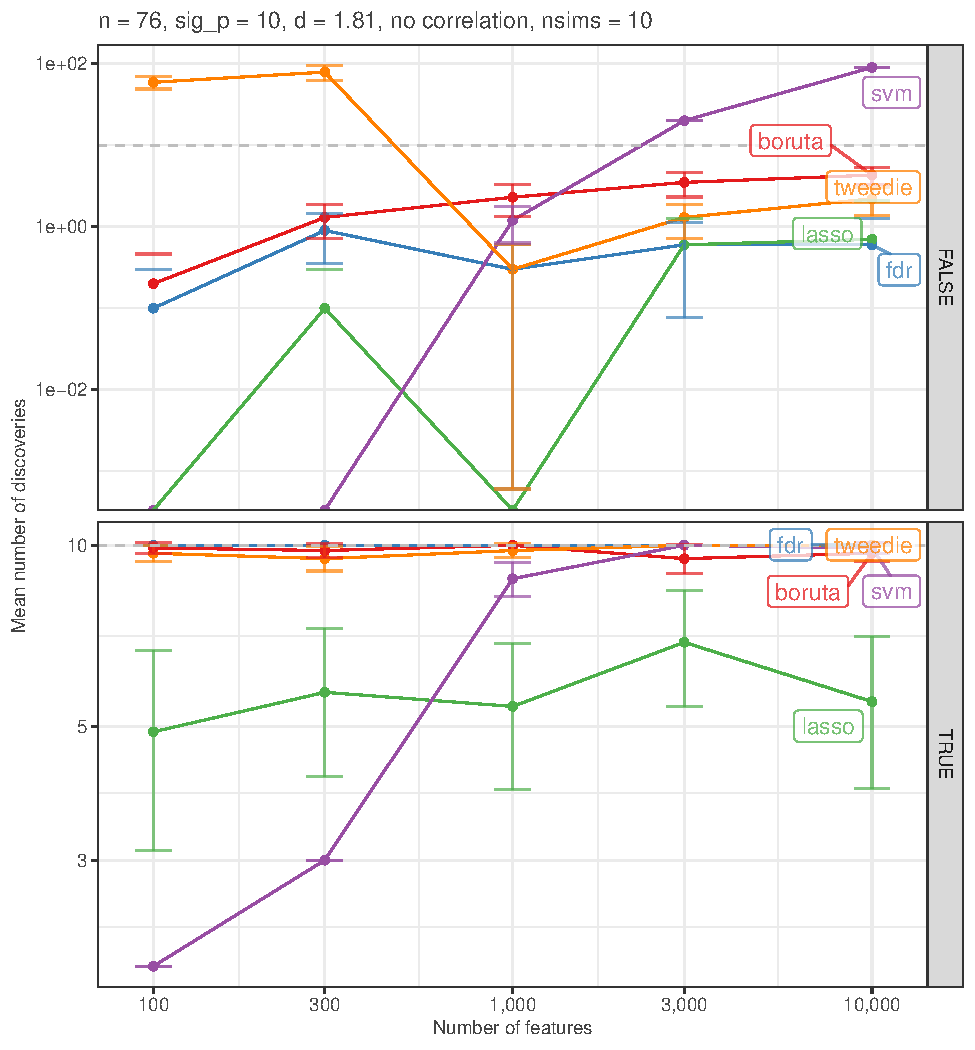
\includegraphics[width=0.49\linewidth]{main_files/figure-latex/unnamed-chunk-7-1} 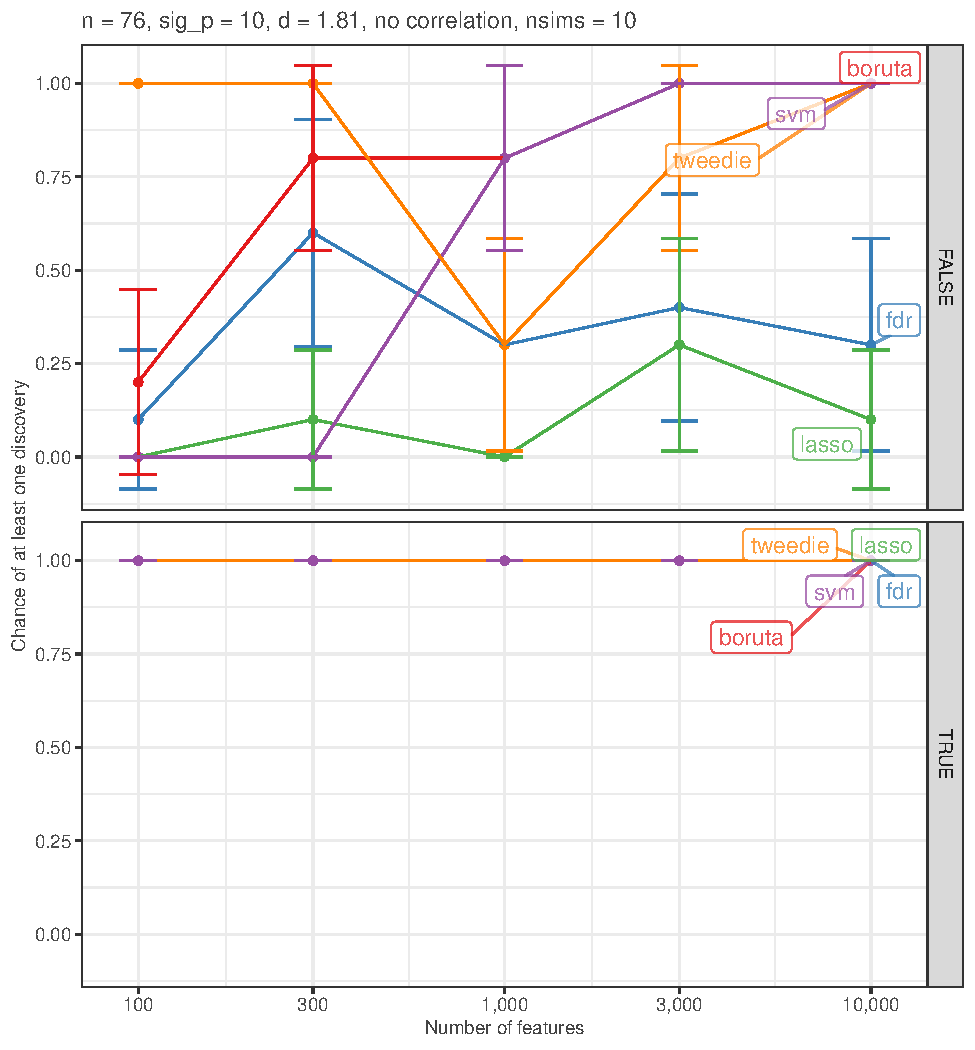
\includegraphics[width=0.49\linewidth]{main_files/figure-latex/unnamed-chunk-7-2} \end{center}

\begin{center}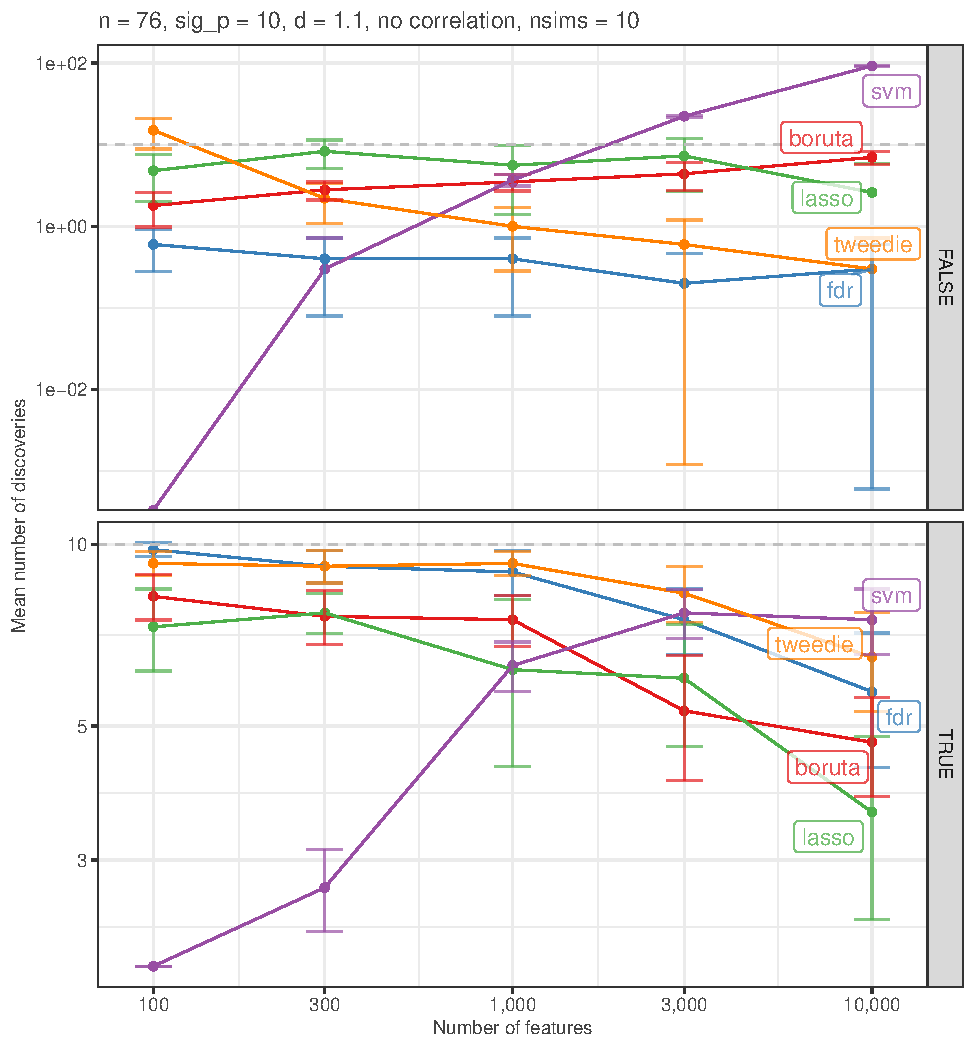
\includegraphics[width=0.49\linewidth]{main_files/figure-latex/unnamed-chunk-8-1} 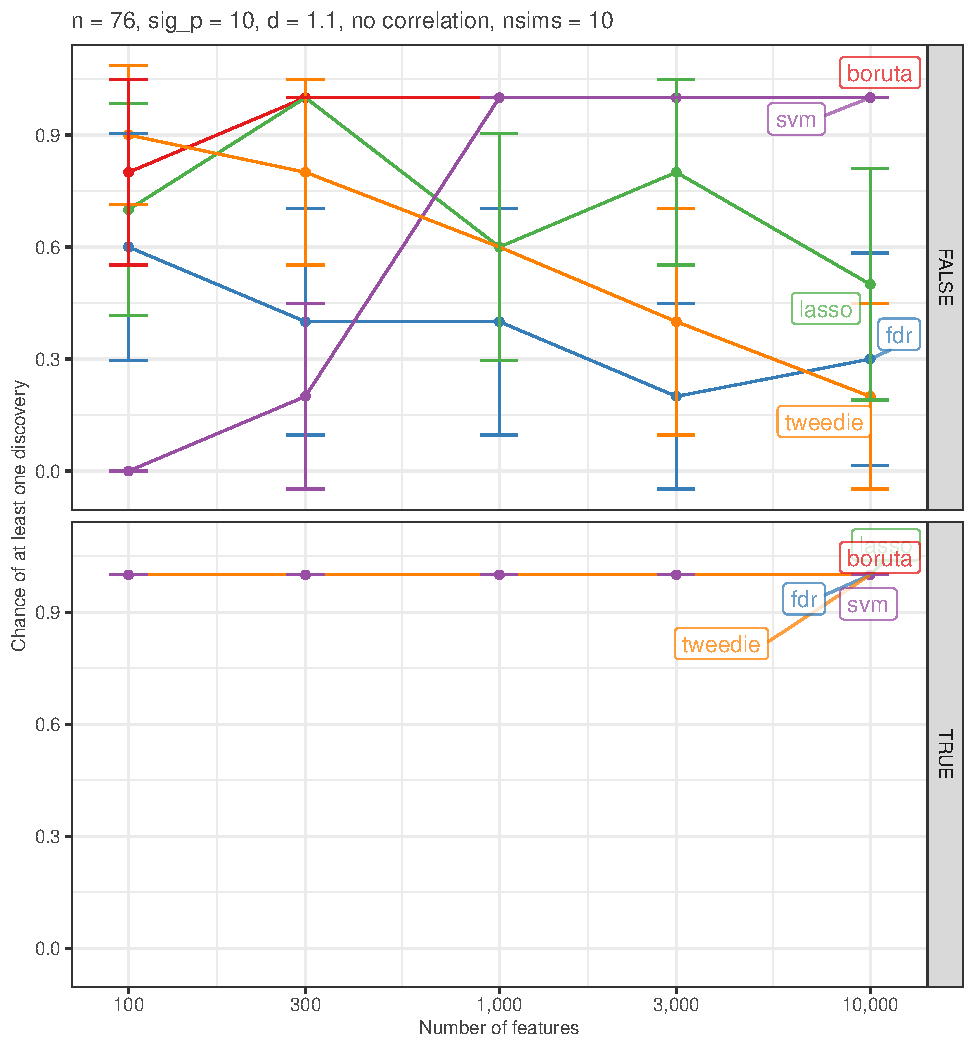
\includegraphics[width=0.49\linewidth]{main_files/figure-latex/unnamed-chunk-8-2} \end{center}

\begin{center}\includegraphics[width=0.49\linewidth]{main_files/figure-latex/unnamed-chunk-9-1} \includegraphics[width=0.49\linewidth]{main_files/figure-latex/unnamed-chunk-9-2} \end{center}

\begin{center}\includegraphics[width=0.49\linewidth]{main_files/figure-latex/unnamed-chunk-10-1} \includegraphics[width=0.49\linewidth]{main_files/figure-latex/unnamed-chunk-10-2} \end{center}

\begin{center}\includegraphics[width=0.49\linewidth]{main_files/figure-latex/unnamed-chunk-11-1} \includegraphics[width=0.49\linewidth]{main_files/figure-latex/unnamed-chunk-11-2} \end{center}

\begin{center}\includegraphics[width=0.49\linewidth]{main_files/figure-latex/unnamed-chunk-12-1} \includegraphics[width=0.49\linewidth]{main_files/figure-latex/unnamed-chunk-12-2} \end{center}

\begin{center}\includegraphics[width=0.49\linewidth]{main_files/figure-latex/unnamed-chunk-13-1} \includegraphics[width=0.49\linewidth]{main_files/figure-latex/unnamed-chunk-13-2} \end{center}

\hypertarget{n-10-sig_p-1-uncorrelated-d-varying}{%
\subsection{n = 10, sig\_p = 1, uncorrelated, d = varying}\label{n-10-sig_p-1-uncorrelated-d-varying}}

\begin{center}\includegraphics[width=0.49\linewidth]{main_files/figure-latex/unnamed-chunk-14-1} \includegraphics[width=0.49\linewidth]{main_files/figure-latex/unnamed-chunk-14-2} \end{center}

\begin{center}\includegraphics[width=0.49\linewidth]{main_files/figure-latex/unnamed-chunk-15-1} \includegraphics[width=0.49\linewidth]{main_files/figure-latex/unnamed-chunk-15-2} \end{center}

\begin{center}\includegraphics[width=0.49\linewidth]{main_files/figure-latex/unnamed-chunk-16-1} \includegraphics[width=0.49\linewidth]{main_files/figure-latex/unnamed-chunk-16-2} \end{center}

\begin{center}\includegraphics[width=0.49\linewidth]{main_files/figure-latex/unnamed-chunk-17-1} \includegraphics[width=0.49\linewidth]{main_files/figure-latex/unnamed-chunk-17-2} \end{center}

\begin{center}\includegraphics[width=0.49\linewidth]{main_files/figure-latex/unnamed-chunk-18-1} \includegraphics[width=0.49\linewidth]{main_files/figure-latex/unnamed-chunk-18-2} \end{center}

\begin{center}\includegraphics[width=0.49\linewidth]{main_files/figure-latex/unnamed-chunk-19-1} \includegraphics[width=0.49\linewidth]{main_files/figure-latex/unnamed-chunk-19-2} \end{center}

\begin{center}\includegraphics[width=0.49\linewidth]{main_files/figure-latex/unnamed-chunk-20-1} \includegraphics[width=0.49\linewidth]{main_files/figure-latex/unnamed-chunk-20-2} \end{center}

\begin{center}\includegraphics[width=0.49\linewidth]{main_files/figure-latex/unnamed-chunk-21-1} \includegraphics[width=0.49\linewidth]{main_files/figure-latex/unnamed-chunk-21-2} \end{center}

\begin{center}\includegraphics[width=0.49\linewidth]{main_files/figure-latex/unnamed-chunk-22-1} \includegraphics[width=0.49\linewidth]{main_files/figure-latex/unnamed-chunk-22-2} \end{center}

\hypertarget{n-30-sig_p-3-uncorrelated-d-varying}{%
\subsection{n = 30, sig\_p = 3, uncorrelated, d = varying}\label{n-30-sig_p-3-uncorrelated-d-varying}}

\begin{center}\includegraphics[width=0.49\linewidth]{main_files/figure-latex/unnamed-chunk-23-1} \includegraphics[width=0.49\linewidth]{main_files/figure-latex/unnamed-chunk-23-2} \end{center}

\begin{center}\includegraphics[width=0.49\linewidth]{main_files/figure-latex/unnamed-chunk-24-1} \includegraphics[width=0.49\linewidth]{main_files/figure-latex/unnamed-chunk-24-2} \end{center}

\begin{center}\includegraphics[width=0.49\linewidth]{main_files/figure-latex/unnamed-chunk-25-1} \includegraphics[width=0.49\linewidth]{main_files/figure-latex/unnamed-chunk-25-2} \end{center}

\begin{center}\includegraphics[width=0.49\linewidth]{main_files/figure-latex/unnamed-chunk-26-1} \includegraphics[width=0.49\linewidth]{main_files/figure-latex/unnamed-chunk-26-2} \end{center}

\begin{center}\includegraphics[width=0.49\linewidth]{main_files/figure-latex/unnamed-chunk-27-1} \includegraphics[width=0.49\linewidth]{main_files/figure-latex/unnamed-chunk-27-2} \end{center}

\begin{center}\includegraphics[width=0.49\linewidth]{main_files/figure-latex/unnamed-chunk-28-1} \includegraphics[width=0.49\linewidth]{main_files/figure-latex/unnamed-chunk-28-2} \end{center}

\begin{center}\includegraphics[width=0.49\linewidth]{main_files/figure-latex/unnamed-chunk-29-1} \includegraphics[width=0.49\linewidth]{main_files/figure-latex/unnamed-chunk-29-2} \end{center}

\begin{center}\includegraphics[width=0.49\linewidth]{main_files/figure-latex/unnamed-chunk-30-1} \includegraphics[width=0.49\linewidth]{main_files/figure-latex/unnamed-chunk-30-2} \end{center}

\begin{center}\includegraphics[width=0.49\linewidth]{main_files/figure-latex/unnamed-chunk-31-1} \includegraphics[width=0.49\linewidth]{main_files/figure-latex/unnamed-chunk-31-2} \end{center}

\begin{center}\includegraphics[width=0.49\linewidth]{main_files/figure-latex/unnamed-chunk-32-1} \includegraphics[width=0.49\linewidth]{main_files/figure-latex/unnamed-chunk-32-2} \end{center}

\hypertarget{sessioninfo}{%
\section{Appendix: Session info}\label{sessioninfo}}

\begin{verbatim}
R version 4.1.1 (2021-08-10)
Platform: x86_64-pc-linux-gnu (64-bit)
Running under: Ubuntu 18.04.5 LTS

Matrix products: default
BLAS:   /usr/lib/x86_64-linux-gnu/blas/libblas.so.3.7.1
LAPACK: /usr/lib/x86_64-linux-gnu/lapack/liblapack.so.3.7.1

locale:
 [1] LC_CTYPE=en_US.UTF-8       LC_NUMERIC=C              
 [3] LC_TIME=en_GB.UTF-8        LC_COLLATE=en_US.UTF-8    
 [5] LC_MONETARY=en_GB.UTF-8    LC_MESSAGES=en_US.UTF-8   
 [7] LC_PAPER=en_GB.UTF-8       LC_NAME=C                 
 [9] LC_ADDRESS=C               LC_TELEPHONE=C            
[11] LC_MEASUREMENT=en_GB.UTF-8 LC_IDENTIFICATION=C       

attached base packages:
[1] parallel  stats     graphics  grDevices utils     datasets  methods  
[8] base     

other attached packages:
 [1] ecolicdf_2.18.0     affy_1.70.0         Biobase_2.52.0     
 [4] BiocGenerics_0.38.0 limma_3.48.3        ggrepel_0.9.1      
 [7] kableExtra_1.3.4    ggcorrplot_0.1.3    forcats_0.5.1      
[10] stringr_1.4.0       dplyr_1.0.6         purrr_0.3.4        
[13] readr_1.4.0         tidyr_1.1.3         tibble_3.1.2       
[16] ggplot2_3.3.3       tidyverse_1.3.1    

loaded via a namespace (and not attached):
 [1] bitops_1.0-7           fs_1.5.0               lubridate_1.7.10      
 [4] bit64_4.0.5            webshot_0.5.2          RColorBrewer_1.1-2    
 [7] httr_1.4.2             GenomeInfoDb_1.28.2    tools_4.1.1           
[10] backports_1.2.1        utf8_1.2.1             R6_2.5.0              
[13] affyio_1.62.0          DBI_1.1.1              colorspace_2.0-1      
[16] withr_2.4.2            tidyselect_1.1.1       bit_4.0.4             
[19] compiler_4.1.1         preprocessCore_1.54.0  cli_2.5.0             
[22] rvest_1.0.0            xml2_1.3.2             labeling_0.4.2        
[25] bookdown_0.22          scales_1.1.1           mvtnorm_1.1-2         
[28] systemfonts_1.0.2      digest_0.6.27          rmarkdown_2.8         
[31] svglite_2.0.0          XVector_0.32.0         pkgconfig_2.0.3       
[34] htmltools_0.5.1.1      fastmap_1.1.0          dbplyr_2.1.1          
[37] rlang_0.4.11           readxl_1.3.1           rstudioapi_0.13       
[40] RSQLite_2.2.8          farver_2.1.0           generics_0.1.0        
[43] jsonlite_1.7.2         RCurl_1.98-1.4         magrittr_2.0.1        
[46] GenomeInfoDbData_1.2.6 S4Vectors_0.30.0       Rcpp_1.0.7            
[49] munsell_0.5.0          fansi_0.5.0            lifecycle_1.0.0       
[52] stringi_1.6.2          yaml_2.2.1             zlibbioc_1.38.0       
[55] plyr_1.8.6             grid_4.1.1             blob_1.2.1            
[58] crayon_1.4.1           Biostrings_2.60.2      haven_2.4.1           
[61] KEGGREST_1.32.0        hms_1.1.0              knitr_1.33            
[64] pillar_1.6.1           reshape2_1.4.4         stats4_4.1.1          
[67] reprex_2.0.0           glue_1.4.2             evaluate_0.14         
[70] BiocManager_1.30.16    modelr_0.1.8           png_0.1-7             
[73] vctrs_0.3.8            cellranger_1.1.0       gtable_0.3.0          
[76] assertthat_0.2.1       cachem_1.0.5           xfun_0.23             
[79] broom_0.7.6            viridisLite_0.4.0      IRanges_2.26.0        
[82] AnnotationDbi_1.54.1   memoise_2.0.0          ellipsis_0.3.2        
\end{verbatim}

\end{document}
